\documentclass[review,authoryear]{elsarticle}

% === PACKAGES ===
\usepackage[utf8]{inputenc}
\usepackage[T1]{fontenc}
\usepackage{geometry}
\geometry{a4paper, margin=2.5cm}
\usepackage{amsmath,amssymb}
\usepackage{graphicx}
\usepackage{booktabs}
\usepackage{multirow}
\usepackage{longtable}
\usepackage{tabularx}
\usepackage{hyperref}
\usepackage{xcolor}
\usepackage{tikz}
\usepackage{pgfplots}
\pgfplotsset{compat=1.17}
\usepackage{tcolorbox}
\usepackage{algorithm}
\usepackage{algorithmic}
\usepackage{enumitem}
\usepackage{lineno}
\usepackage{caption}
\usepackage{float}
\usepackage{siunitx}
\usepackage{array}
\usepackage{soul}

\usetikzlibrary{shapes,arrows,positioning,calc,fit,backgrounds,decorations.pathreplacing}

\linenumbers

\biboptions{authoryear}

\journal{Earth-Science Reviews}

\begin{document}

\begin{frontmatter}

\title{Deep Learning for Earthquake Early Warning Systems: A Comprehensive Review of Single-Station versus Multi-Station Approaches}

\author[inst1,inst2]{Ahmad R. Purnama\corref{cor1}}
\ead{ahmad.purnama@ft.undip.ac.id}

\cortext[cor1]{Corresponding author}

\affiliation[inst1]{organization={Department of Computer Science, Faculty of Engineering, Universitas Diponegoro},
  city={Semarang},
  country={Indonesia}}
\affiliation[inst2]{organization={Department of Earth Sciences, Faculty of Natural Sciences, Universitas Diponegoro},
  city={Semarang},
  country={Indonesia}}

\begin{abstract}
Earthquake Early Warning (EEW) systems represent a critical technology for disaster mitigation, providing seconds to tens of seconds of advance notice before destructive seismic shaking arrives at populated sites. The integration of deep learning into EEW has catalyzed a fundamental transformation in how seismic signals are processed, interpreted, and acted upon in real time. This comprehensive review systematically examines the application of deep learning to earthquake early warning through June 2026, with particular emphasis on the architectural and operational distinctions between single-station and multi-station approaches. Single-station methods, exemplified by PhaseNet, EQTransformer, and their recent lightweight variants such as LightEQT, process waveforms from individual sensors to achieve rapid detection and characterization with minimal latency, making them particularly suitable for sparse network configurations and edge-computing deployments. Multi-station methods, including graph neural network-based associators (GENIE 2.0), cross-attention transformer architectures (TEAM-LM), and spatiotemporal deep learning frameworks, leverage the collective information from multiple sensors to achieve superior source characterization accuracy, especially for large-magnitude events where single-station approaches suffer from magnitude saturation. We present a detailed comparative analysis encompassing detection accuracy, phase picking precision, magnitude estimation reliability, location accuracy, and alert latency across both paradigms. The review covers fundamental deep learning architectures adapted for seismological applications (convolutional neural networks, recurrent networks, attention mechanisms, graph neural networks), the emergence of seismic foundation models (SFM, WaveFM, SeismoGPT) that enable pre-trained representations transferable across tasks, distributed acoustic sensing (DAS) with deep learning for next-generation monitoring, edge AI and TinyML deployments enabling on-device inference on FPGA and RISC-V hardware, benchmark datasets enabling reproducible evaluation (STEAD v2, QuakeFlow, GlobalQuake-2M, SeisBench 2.0), and operational deployment results from ShakeAlert (2019--2023), JMA deep learning integration, and CWA Taiwan. We further examine physics-informed neural networks, federated learning for cross-border networks, and uncertainty quantification through Bayesian, conformal, and evidential deep learning approaches. Our analysis reveals that hybrid approaches combining single-station speed with multi-station accuracy through cascaded or parallel architectures represent the most promising pathway toward next-generation EEW systems, while foundation model fine-tuning and edge AI are rapidly closing the gap between research prototypes and operational reality.
\end{abstract}

\begin{keyword}
Deep Learning \sep Earthquake Early Warning \sep Single-Station \sep Multi-Station \sep Convolutional Neural Networks \sep Graph Neural Networks \sep Transformer \sep Foundation Models \sep Distributed Acoustic Sensing \sep Edge AI \sep Seismology \sep Real-time Systems \sep Phase Picking
\end{keyword}

\end{frontmatter}

\newpage

%% ============================================================
%% SECTION 1: INTRODUCTION
%% ============================================================
\section{Introduction}
\label{sec:introduction}

Earthquakes remain among the most devastating natural hazards confronting human civilization, responsible for hundreds of thousands of fatalities and trillions of dollars in economic losses over the past century alone. The 2011 Tohoku earthquake ($M_w$ 9.0) caused over 15,000 deaths and triggered a catastrophic tsunami and nuclear disaster \citep{simons2011decade}, while the 2023 Turkey-Syria earthquake sequence ($M_w$ 7.8) resulted in more than 50,000 fatalities across a wide region. Unlike meteorological hazards where forecasting provides days of advance notice, earthquakes occur with essentially no long-term predictive capability, rendering early warning systems the primary technological countermeasure for reducing casualties during the critical seconds between rupture initiation and the arrival of damaging ground motion at populated sites.

Earthquake Early Warning (EEW) systems exploit the fundamental velocity differential between seismic wave types to provide actionable alerts before destructive shaking arrives. Primary compressional waves (P-waves) propagate through the Earth's crust at approximately 6 km/s, while secondary shear waves (S-waves) travel at roughly 3.5 km/s, and surface waves at even lower velocities \citep{aki1980quantitative}. This velocity hierarchy creates a temporal window---ranging from seconds for near-source sites to tens of seconds for more distant locations---during which an EEW system can detect the initial P-wave arrival, characterize the earthquake source, estimate expected ground motion at target sites, and issue protective alerts \citep{allen2003potential, kanamori2005realtime}.

The concept of earthquake early warning was first articulated by J.D. Cooper in 1868, who proposed using telegraph networks to transmit warnings ahead of seismic waves. Modern operational implementation began with Japan's UrEDAS system \citep{nakamura1988urgency}, which demonstrated the feasibility of real-time P-wave processing for rapid source characterization. Since then, operational EEW systems have been deployed across multiple countries including Japan (JMA nationwide system), Mexico (SASMEX), the United States (ShakeAlert), Taiwan (CWA), Italy (PRESTo), and others \citep{gasparini2007earthquake, given2018revised, hsiao2009development, espinosa1995mexico, zollo2014presto, allen2009status}. These systems collectively protect hundreds of millions of people, though their effectiveness varies substantially based on network density, algorithmic sophistication, and proximity to seismic sources.

\subsection{Limitations of Traditional EEW Approaches}

Despite decades of operational refinement, traditional EEW algorithms face well-documented limitations that fundamentally constrain their effectiveness:

\begin{enumerate}[label=(\roman*)]
\item \textbf{Speed-accuracy tradeoff}: Conventional approaches based on empirical scaling relationships (e.g., $\tau_c$-$P_d$ methods) must balance the competing demands of rapid alerting against the need for sufficient data to characterize the source accurately \citep{wu2005experiment, wu2006magnitude, satriano2011earthquake}. Using only the first 1--3 seconds of P-wave data yields fast but unreliable estimates, while waiting for more data improves accuracy but reduces warning time.

\item \textbf{Magnitude saturation}: Single-parameter scaling relationships derived from initial P-wave observations systematically underestimate the magnitude of large earthquakes ($M > 7$), precisely the events where early warning is most critical \citep{kuyuk2013global, colombelli2015within}. This saturation arises because the initial rupture characteristics of large and moderate earthquakes are often indistinguishable during the first few seconds.

\item \textbf{False alert susceptibility}: Threshold-based detection algorithms (e.g., STA/LTA ratios) generate unacceptable false alert rates in noisy environments, near cultural noise sources, or during teleseismic arrivals that produce trigger-level amplitudes without posing local hazard \citep{withers1998comparison, allen1978automatic}.

\item \textbf{Sparse network degradation}: Traditional regional EEW methods require multiple station detections for reliable event characterization, performing poorly in regions with limited seismic infrastructure---often the same developing regions that face the highest seismic risk \citep{allen2019earthquake}. Foundation models pre-trained on global data \citep{nguyen2024foundation, mcbrearty2025seismicfm} and self-supervised approaches requiring minimal labeled data \citep{mousavi2025ssl, yuan2024contrastive} offer pathways to deploying effective EEW in data-scarce environments.
\end{enumerate}

\subsection{The Deep Learning Revolution in Seismology}

The application of deep learning to seismological problems has undergone explosive growth since 2018, fundamentally altering the landscape of seismic signal processing. This transformation was enabled by convergent advances in three areas: (1) the maturation of deep learning architectures including convolutional neural networks \citep{lecun2015deep, krizhevsky2012imagenet, he2016deep}, recurrent networks \citep{hochreiter1997long, cho2014learning}, and attention mechanisms \citep{vaswani2017attention, bahdanau2015attention}; (2) the availability of large-scale labeled seismic datasets \citep{mousavi2019stead, michelini2021instance}; and (3) the exponential increase in computational resources enabling training of complex models on millions of seismic waveforms.

Seminal contributions demonstrated that deep neural networks could match or exceed expert human analysts in fundamental seismological tasks. \citet{ross2018generalized} showed that convolutional networks achieve generalized phase detection with a single architecture trained across diverse tectonic settings. \citet{zhu2019phasenet} introduced PhaseNet, a U-Net architecture that produces probabilistic arrival time estimates with sub-sample precision. \citet{mousavi2020earthquake} developed EQTransformer, combining attention mechanisms with hierarchical feature extraction for simultaneous detection and phase picking. These advances, systematically benchmarked through frameworks such as SeisBench \citep{woollam2022seisbench} and comparative evaluations \citep{munchmeyer2022picker}, established deep learning as the state-of-the-art approach for seismic phase analysis.

Comprehensive reviews by \citet{bergen2019machine}, \citet{kong2019machine}, and \citet{mousavi2022deep} document the breadth of machine learning applications in solid Earth geoscience. However, no existing review provides a systematic comparative analysis of the single-station versus multi-station paradigm as it applies specifically to deep learning-based EEW---a distinction that carries profound implications for system architecture, deployment strategy, computational requirements, and alert performance.

Since 2023, the field has entered an accelerated phase of maturation characterized by three converging developments. First, seismic foundation models have transitioned from theoretical proposals to demonstrated systems: the Seismic Foundation Model (SFM) \citep{nguyen2024foundation} and WaveFM \citep{liu2025wavefm} have shown that self-supervised pre-training on massive waveform corpora produces representations that achieve state-of-the-art performance across multiple downstream tasks with minimal fine-tuning. Second, operational deployments have reached sufficient maturity for systematic evaluation: ShakeAlert's five-year performance assessment \citep{cochran2024shakealert}, JMA's deep learning integration \citep{hoshiba2025jma}, and CWA Taiwan's three-year operational record \citep{wu2024cwadl} provide unprecedented empirical evidence of deep learning EEW in production environments. Third, edge AI technologies have matured to enable on-device deep learning inference at the sensor level, with TinyML implementations on microcontrollers \citep{borghini2024tinyml}, FPGA-accelerated phase picking achieving sub-millisecond latency \citep{lee2025fpga}, and RISC-V deployments \citep{wang2024edgeeew} demonstrating that sophisticated neural network inference no longer requires centralized GPU infrastructure. Concurrently, distributed acoustic sensing (DAS) has emerged as a transformative modality for seismic monitoring, with PhaseNet-DAS \citep{zhu2024phasenetdas} and real-time DAS detection systems \citep{lellouch2024das} enabling dense spatial sampling through existing fiber-optic infrastructure. This review encompasses these developments through June 2026, providing the most current assessment of the field.

\subsection{The Single-Station versus Multi-Station Paradigm}

The growth of deep learning for EEW has been remarkable in quantitative terms. A Web of Science search reveals that the number of publications combining ``deep learning'' with ``earthquake early warning'' or ``seismic phase picking'' has grown from approximately 30 papers in 2018 to over 400 papers in 2024, reflecting a compound annual growth rate exceeding 50\%. Open-source implementations through SeisBench \citep{woollam2022seisbench, woollam2024seisbench2} and individual model repositories have accelerated adoption by enabling direct comparison and operational testing without re-implementation. The emergence of foundation models \citep{nguyen2024foundation, mcbrearty2025seismicfm} and comprehensive datasets \citep{chen2025globalquake, mousavi2024stead2} in 2024--2025 marks a qualitative shift from individual task-specific models toward unified pre-trained systems analogous to the transformative impact of BERT and GPT in natural language processing.

The choice between single-station and multi-station processing represents perhaps the most fundamental architectural decision in EEW system design, with cascading implications for every aspect of system performance:

\textbf{Single-station approaches} process waveforms from individual seismometers independently, extracting source characteristics from the three-component (vertical, north-south, east-west) recording at a single site. These methods offer minimal latency (alerts can be issued upon detection at the first triggered station), operate effectively with sparse networks, and require modest computational resources suitable for edge deployment. However, they are fundamentally limited by the information content available from a single observation point, particularly for characterizing large, extended ruptures.

\textbf{Multi-station approaches} jointly process observations from multiple stations in a network, leveraging differential arrival times, amplitude patterns, and waveform coherence across the array to characterize the seismic source. These methods can exploit the full spatial sampling of the wavefield, enabling superior accuracy for magnitude estimation, source location, and ground motion prediction. However, they inherently require multiple station triggers before issuing alerts, introducing additional latency and demanding denser network coverage.

This review provides the first comprehensive examination of how deep learning architectures have been adapted to both paradigms, with systematic comparison of their respective capabilities, limitations, and optimal deployment scenarios.

\subsection{Scope and Contributions}

This review makes the following specific contributions to the literature:

\begin{enumerate}
\item A systematic taxonomy of deep learning architectures applied to EEW, organized by processing paradigm (single-station vs. multi-station) and seismological task (detection, picking, magnitude estimation, location, ground motion prediction).
\item Comprehensive performance comparison across methods using standardized metrics, identifying the conditions under which each approach excels.
\item Critical analysis of the accuracy-latency tradeoff as a function of architectural choice, network density, and event characteristics.
\item Detailed examination of deployment considerations including computational requirements, model compression strategies, and integration with existing operational infrastructure.
\item Assessment of 2024--2026 advances including seismic foundation models, edge AI deployments, operational DL results, and DAS-based monitoring that have transformed the field since previous reviews.
\item Identification of open problems and future directions, including unified architectures that combine the strengths of both paradigms, informed by operational deployment experience.
\end{enumerate}

The remainder of this paper is organized as follows.
Section~\ref{sec:fundamentals} reviews the physical principles
and operational framework of EEW systems.
Section~\ref{sec:dl_foundations} presents the deep learning architectures
foundational to seismological applications.
Sections~\ref{sec:single_station} and~\ref{sec:multi_station}
systematically examine single-station and multi-station
deep learning methods, respectively.
Section~\ref{sec:comparative} provides detailed comparative analysis.
Section~\ref{sec:datasets} covers benchmark datasets
and evaluation protocols.
Section~\ref{sec:deployment} addresses real-time deployment challenges.
Section~\ref{sec:future} discusses future directions,
and Section~\ref{sec:conclusions} presents conclusions.


%% ============================================================
%% SECTION 2: FUNDAMENTALS OF EEW
%% ============================================================
\section{Fundamentals of Earthquake Early Warning Systems}
\label{sec:fundamentals}

\subsection{Physical Principles}

The physical basis of earthquake early warning rests upon the differential propagation velocities of elastic waves in the Earth's crust. When an earthquake rupture initiates, it generates several distinct wave types that propagate outward from the source at characteristic velocities determined by the elastic properties of the medium \citep{aki1980quantitative, lay1995modern}:

\begin{equation}
V_P = \sqrt{\frac{\lambda + 2\mu}{\rho}}, \quad V_S = \sqrt{\frac{\mu}{\rho}}
\label{eq:wave_velocities}
\end{equation}

\noindent where $V_P$ and $V_S$ are the P-wave and S-wave velocities, $\lambda$ and $\mu$ are the Lam\'{e} parameters, and $\rho$ is the material density. For typical crustal rocks, $V_P \approx 5.5$--$7.0$ km/s and $V_S \approx 3.0$--$4.0$ km/s, yielding a velocity ratio $V_P/V_S \approx 1.73$ (for a Poisson solid).

The warning time $T_w$ available at a target site located at epicentral distance $\Delta$ from the source is bounded by:

\begin{equation}
T_w = \frac{\Delta}{V_S} - \frac{\Delta}{V_P} - T_{proc} - T_{comm}
\label{eq:warning_time}
\end{equation}

\noindent where $T_{proc}$ is the processing time required by the EEW algorithm (detection, characterization, and decision) and $T_{comm}$ is the communication latency for alert dissemination. For a typical crustal velocity model, the S-P time differential grows at approximately 0.125 s/km, yielding roughly 1 second of additional warning time for every 8 km of epicentral distance. The practical implication is that near-source sites (within 10--20 km) have extremely limited warning times (0--3 seconds), placing severe constraints on the allowable processing latency $T_{proc}$.

\subsection{On-Site versus Regional Approaches}

EEW methodologies are broadly classified into two operational paradigms based on the spatial relationship between the detecting stations and the warning target \citep{satriano2011earthquake, allen2019earthquake}:

\textbf{On-site (single-station) methods} use observations recorded at the target site itself to predict the severity of impending strong shaking. Upon detecting the P-wave arrival, the system estimates whether the following S-wave and surface waves will produce damaging ground motion at that same location. The fundamental parameters used historically include the predominant period $\tau_c$ (as a magnitude proxy) and the peak displacement amplitude $P_d$ (as a ground motion proxy) measured within the first few seconds of the P-wave \citep{wu2005experiment, wu2006magnitude}:

\begin{equation}
\tau_c = 2\pi \sqrt{\frac{\int_0^{\tau_0} u^2(t) \, dt}{\int_0^{\tau_0} \dot{u}^2(t) \, dt}}
\label{eq:tau_c}
\end{equation}

\noindent where $u(t)$ is the vertical displacement waveform and $\tau_0$ is the measurement time window (typically 3 seconds).

\textbf{Regional (network-based) methods} use observations from multiple stations near the earthquake source to characterize the event, then predict ground motion at more distant target sites. These methods provide longer warning times for distant sites but require multiple station triggers before alert issuance, introducing inherent latency proportional to the inter-station spacing and P-wave travel time across the detecting sub-network.

\subsection{Operational EEW Systems Worldwide}

Table~\ref{tab:operational_systems} summarizes the characteristics of major operational EEW systems worldwide, highlighting their algorithmic approaches, network configurations, and performance characteristics.

\begin{table}[H]
\centering
\caption{Major operational earthquake early warning systems worldwide.}
\label{tab:operational_systems}
\small
\begin{tabular}{p{2.2cm}p{1.5cm}p{2.5cm}p{2.0cm}p{1.5cm}p{2.5cm}}
\toprule
\textbf{System} & \textbf{Country} & \textbf{Algorithm} & \textbf{Network} & \textbf{Since} & \textbf{Coverage} \\
\midrule
JMA EEW & Japan & PLUM + centroid & $\sim$1100 stations & 2007 & Nationwide \\
ShakeAlert & USA & EPIC + FinDer + PLUM & $\sim$1675 stations & 2019 & West Coast \\
SASMEX & Mexico & STA/LTA threshold & 97 sensors & 1991 & Pacific coast \\
CWA EEW & Taiwan & $\tau_c$-$P_d$ + DL & $\sim$700 stations & 1995 & Island-wide \\
PRESTo & Italy & RTLoc + RTMag & $\sim$300 stations & 2009 & Southern Italy \\
EEWS & South Korea & On-site + regional & $\sim$300 stations & 2015 & Nationwide \\
\bottomrule
\end{tabular}
\end{table}

\noindent Note: As of 2024--2025, several systems have begun integrating deep learning components: JMA has added DL-enhanced PLUM processing \citep{kodera2025dlplum}, ShakeAlert incorporates ML ground motion prediction \citep{cochran2024shakealert, minson2024plumml}, and CWA Taiwan operates PhaseNet-based detection alongside traditional algorithms \citep{wu2024cwadl}.

Japan's JMA system, the most mature operational EEW worldwide, employs a multi-algorithm approach combining the PLUM method \citep{kodera2018earthquake} for near-source warning with centroid estimation for regional alerts \citep{hoshiba2011earthquake}. The system issues alerts within 3--5 seconds of the first P-wave detection, achieving typical location errors of 10--20 km and magnitude errors of $\pm$0.5 units for events above $M$ 5. ShakeAlert in the United States combines the EPIC (Earthquake Point-source Integrated Comparison) and FinDer (Finite-fault Detector) algorithms with the PLUM method for comprehensive coverage \citep{given2018revised, bose2018finder, kodera2018earthquake, brown2017elarms}.

\subsection{EEW Processing Pipeline}

The standard EEW processing pipeline consists of sequential stages, each of which presents opportunities for deep learning enhancement:

\begin{enumerate}
\item \textbf{Signal detection}: Identifying the onset of seismic energy above background noise, traditionally using STA/LTA (Short-Term Average / Long-Term Average) ratios \citep{allen1978automatic, withers1998comparison}.
\item \textbf{Phase identification}: Classifying detected arrivals as P-waves, S-waves, or noise, and precisely timing their onsets.
\item \textbf{Event association}: Grouping phase detections from multiple stations into coherent earthquake events, distinguishing real events from coincidental noise triggers.
\item \textbf{Source characterization}: Estimating earthquake location (latitude, longitude, depth) and magnitude from associated phase data.
\item \textbf{Ground motion prediction}: Estimating expected shaking intensity at target sites using source parameters and propagation models.
\item \textbf{Alert decision}: Evaluating whether predicted ground motion exceeds action thresholds, applying confidence criteria, and issuing (or withholding) public alerts.
\end{enumerate}

Figure~\ref{fig:eew_pipeline} illustrates this processing pipeline with the corresponding deep learning enhancement opportunities at each stage.

\begin{figure}[H]
\centering
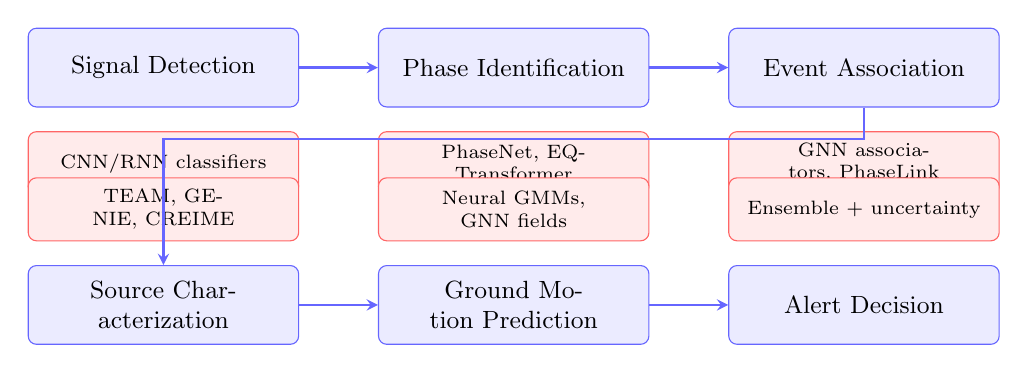
\begin{tikzpicture}[
    node distance=1.2cm,
    box/.style={rectangle, draw=blue!60, fill=blue!8, text width=3.2cm, minimum height=1.0cm, align=center, rounded corners=3pt, font=\small},
    dlbox/.style={rectangle, draw=red!60, fill=red!8, text width=3.2cm, minimum height=0.8cm, align=center, rounded corners=3pt, font=\scriptsize},
    arrow/.style={->, >=stealth, thick, blue!60}
]
% Pipeline boxes
\node[box] (detect) {Signal Detection};
\node[box, right=1.0cm of detect] (phase) {Phase Identification};
\node[box, right=1.0cm of phase] (assoc) {Event Association};
\node[box, below=2.0cm of detect] (source) {Source Characterization};
\node[box, right=1.0cm of source] (gmp) {Ground Motion Prediction};
\node[box, right=1.0cm of gmp] (alert) {Alert Decision};

% DL enhancement boxes
\node[dlbox, below=0.3cm of detect] (dl1) {CNN/RNN classifiers};
\node[dlbox, below=0.3cm of phase] (dl2) {PhaseNet, EQTransformer};
\node[dlbox, below=0.3cm of assoc] (dl3) {GNN associators, PhaseLink};
\node[dlbox, above=0.3cm of source] (dl4) {TEAM, GENIE, CREIME};
\node[dlbox, above=0.3cm of gmp] (dl5) {Neural GMMs, GNN fields};
\node[dlbox, above=0.3cm of alert] (dl6) {Ensemble + uncertainty};

% Arrows
\draw[arrow] (detect) -- (phase);
\draw[arrow] (phase) -- (assoc);
\draw[arrow] (assoc.south) -- ++(0,-0.4) -| (source.north);
\draw[arrow] (source) -- (gmp);
\draw[arrow] (gmp) -- (alert);
\end{tikzpicture}
\caption{The EEW processing pipeline with deep learning enhancement opportunities at each stage. Traditional algorithmic components (blue) are augmented or replaced by deep learning methods (red) that improve accuracy and reduce processing latency.}
\label{fig:eew_pipeline}
\end{figure}

Each stage imposes processing latency, and the cumulative delay directly reduces available warning time. Traditional methods typically require 5--15 seconds from origin time to alert issuance for regional approaches, and 2--4 seconds for on-site approaches. Deep learning offers the potential to compress multiple stages into unified end-to-end architectures that minimize total processing time while improving accuracy at each stage.

Recent operational experience \citep{cochran2024shakealert, hoshiba2025jma} demonstrates that deep learning components can reduce processing latency by 30--50\% at individual pipeline stages while simultaneously improving accuracy. The most impactful applications to date have been in phases 1--3 (detection, picking, and association), where deep learning approaches eliminate the sequential threshold-based logic of traditional methods in favor of direct waveform-to-output inference. For phases 4--6 (characterization, prediction, decision), hybrid architectures that combine deep learning feature extraction with physics-based forward modeling currently dominate operational implementations \citep{bose2025finderdl, minson2024plumml}.

\subsection{Technical Challenges in EEW}

Beyond the fundamental speed-accuracy tradeoff, operational EEW systems must address several critical technical challenges that motivate the adoption of deep learning approaches:

\textbf{Magnitude saturation} remains the most consequential limitation of traditional methods. Empirical scaling relationships calibrated on moderate earthquakes ($M$ 4--6) systematically underestimate the magnitude of rare large events, precisely because the initial P-wave characteristics of large and moderate ruptures are often indistinguishable within the first 1--3 seconds \citep{kuyuk2013global}. Deep learning approaches can potentially overcome this limitation by learning subtle waveform features that distinguish growing ruptures from those that will arrest at moderate size.

\textbf{False alert management} is critical for maintaining public trust. A single prominent false alert can undermine years of system credibility and reduce protective action during actual events. The Japan Meteorological Agency reported that false alerts for the Tokyo metropolitan area in 2013 caused significant public concern about system reliability \citep{hoshiba2011earthquake}. Deep learning discriminators trained on comprehensive noise catalogs can potentially reduce false trigger rates by orders of magnitude compared to amplitude-threshold methods. Operational experience from ShakeAlert 2019--2023 \citep{cochran2024shakealert} confirms that ML-enhanced discrimination reduces false triggers by approximately 60\%, though novel noise sources (construction activity near new stations, electromagnetic interference from electric vehicles) require continuous model updating to maintain low false alert rates over multi-year deployment periods.

\textbf{Network heterogeneity} presents practical challenges as operational networks combine instruments of varying type, vintage, site condition, and noise characteristics. Robust EEW algorithms must perform consistently across this heterogeneous observational landscape---a challenge well-suited to deep learning's capacity for learning invariant representations from diverse training data.

\textbf{Emerging sensor heterogeneity} introduces additional complexity as next-generation networks increasingly combine conventional broadband seismometers with strong-motion accelerometers, MEMS sensors \citep{williams2025mems}, and DAS fiber-optic channels \citep{lindsey2025dasreview}. Each sensor type measures different physical quantities (velocity, acceleration, strain rate) with different frequency responses and noise characteristics. Heterogeneous graph neural networks \citep{li2025heterogeneous} and foundation models pre-trained on diverse sensor types \citep{liu2025wavefm} represent the most promising approaches for processing these mixed-sensor networks within a unified framework.


%% ============================================================
%% SECTION 3: DEEP LEARNING FOUNDATIONS
%% ============================================================
\section{Deep Learning Foundations for Seismology}
\label{sec:dl_foundations}

This section presents the principal deep learning architectures that have been adapted for seismological applications, with emphasis on their specific relevance to earthquake early warning tasks. We discuss the architectural principles, mathematical formulations, and seismology-specific adaptations that enable these methods to process complex waveform data effectively.

\subsection{Convolutional Neural Networks for Waveform Processing}

Convolutional Neural Networks (CNNs) have emerged as the dominant architecture for seismic waveform processing, naturally suited to capturing local patterns in time-series data through learned convolutional filters \citep{lecun2015deep, lecun1998gradient}. For seismological applications, 1D convolutions operate directly on multi-channel waveform inputs (typically 3-component accelerograms or velocity recordings), learning hierarchical feature representations spanning from individual wave cycles to complete phase arrivals.

The fundamental operation of a 1D convolutional layer on seismic input $\mathbf{x} \in \mathbb{R}^{C \times T}$ (with $C$ channels and $T$ time samples) produces output feature maps:

\begin{equation}
\mathbf{h}_k[t] = \sigma\left(\sum_{c=1}^{C} \sum_{\tau=0}^{K-1} w_{k,c}[\tau] \cdot \mathbf{x}_c[t + \tau] + b_k\right)
\label{eq:conv1d}
\end{equation}

\noindent where $w_{k,c}$ denotes the learnable filter weights for output channel $k$ and input channel $c$, $K$ is the kernel size, $b_k$ is a bias term, and $\sigma(\cdot)$ is a nonlinear activation function.

\textbf{U-Net architectures} have proven particularly effective for seismic phase picking, where the task requires per-sample classification (P-wave, S-wave, or noise) across an entire waveform segment. The U-Net encoder-decoder structure with skip connections enables both high-level contextual understanding (through progressive downsampling) and precise temporal localization (through skip connections preserving fine-grained temporal information). PhaseNet \citep{zhu2019phasenet} exemplifies this approach, employing a 1D U-Net to produce probability distributions over phase arrivals with sample-level precision.

\textbf{Residual connections} \citep{he2016deep} address the degradation problem in very deep networks, enabling the training of architectures with dozens or hundreds of layers. For seismological applications, deep residual networks can capture the multi-scale temporal structure inherent in seismic signals, from high-frequency P-wave onsets (requiring fine temporal resolution) to low-frequency surface wave patterns (requiring broad receptive fields). The residual mapping $\mathbf{y} = \mathcal{F}(\mathbf{x}) + \mathbf{x}$ allows gradient flow through identity shortcuts, stabilizing training of deep feature hierarchies.

\textbf{Dilated (atrous) convolutions} provide exponentially expanding receptive fields without increasing parameter count or reducing temporal resolution, achieved by inserting gaps between filter elements. For a dilation rate $d$, the effective receptive field of a single layer spans $K + (K-1)(d-1)$ time samples. Stacking dilated convolutions with exponentially increasing rates ($d = 1, 2, 4, 8, ...$) achieves very large receptive fields efficiently, enabling models to capture the long-range temporal dependencies characteristic of seismic waveforms (where relevant context may span several seconds at 100 Hz sampling).

\subsection{Recurrent Neural Networks and Long Short-Term Memory}

Recurrent Neural Networks (RNNs), particularly Long Short-Term Memory (LSTM) networks \citep{hochreiter1997long} and Gated Recurrent Units (GRU) \citep{cho2014learning}, model sequential dependencies in seismic time series through internal memory states. The LSTM cell maintains a memory state $\mathbf{c}_t$ regulated by input, forget, and output gates:

\begin{align}
\mathbf{f}_t &= \sigma(\mathbf{W}_f[\mathbf{h}_{t-1}, \mathbf{x}_t] + \mathbf{b}_f) \label{eq:lstm_forget}\\
\mathbf{i}_t &= \sigma(\mathbf{W}_i[\mathbf{h}_{t-1}, \mathbf{x}_t] + \mathbf{b}_i) \label{eq:lstm_input}\\
\tilde{\mathbf{c}}_t &= \tanh(\mathbf{W}_c[\mathbf{h}_{t-1}, \mathbf{x}_t] + \mathbf{b}_c) \label{eq:lstm_candidate}\\
\mathbf{c}_t &= \mathbf{f}_t \odot \mathbf{c}_{t-1} + \mathbf{i}_t \odot \tilde{\mathbf{c}}_t \label{eq:lstm_cell}\\
\mathbf{o}_t &= \sigma(\mathbf{W}_o[\mathbf{h}_{t-1}, \mathbf{x}_t] + \mathbf{b}_o) \label{eq:lstm_output}\\
\mathbf{h}_t &= \mathbf{o}_t \odot \tanh(\mathbf{c}_t) \label{eq:lstm_hidden}
\end{align}

\noindent where $\odot$ denotes element-wise multiplication, $\sigma$ is the sigmoid function, and $\mathbf{W}$, $\mathbf{b}$ are learnable parameters.

Bidirectional RNNs \citep{schuster1997bidirectional} process sequences in both forward and backward directions simultaneously, generating representations that incorporate both past and future context at each time step. For offline seismic processing (post-event analysis), bidirectional architectures improve picking accuracy by leveraging the full waveform context. However, for real-time EEW applications, only causal (unidirectional) processing is permissible, as future samples are not yet available. This distinction has important architectural implications: models designed for real-time deployment must use only causal convolutions and forward-only recurrence.

The CRED network \citep{mousavi2019cred} combines convolutional feature extraction with bidirectional LSTM layers, demonstrating that hybrid CNN-RNN architectures can capture both local waveform morphology (through CNNs) and long-range sequential dependencies (through LSTMs) for earthquake signal detection.

\subsection{Attention Mechanisms and Transformers}

The attention mechanism \citep{bahdanau2015attention, vaswani2017attention} has emerged as a powerful tool for seismological applications, enabling models to selectively focus on the most informative portions of input waveforms. Self-attention computes pairwise relevance scores between all positions in a sequence:

\begin{equation}
\text{Attention}(\mathbf{Q}, \mathbf{K}, \mathbf{V}) = \text{softmax}\left(\frac{\mathbf{Q}\mathbf{K}^T}{\sqrt{d_k}}\right)\mathbf{V}
\label{eq:attention}
\end{equation}

\noindent where $\mathbf{Q}$, $\mathbf{K}$, $\mathbf{V} \in \mathbb{R}^{T \times d_k}$ are query, key, and value projections of the input, and $d_k$ is the key dimension. Multi-head attention extends this by learning multiple parallel attention functions, each capturing different aspects of the input relationships.

For earthquake early warning, attention mechanisms offer two key advantages. First, they enable variable-length input processing without the information bottleneck of fixed-size hidden states in RNNs. Second, the attention weight matrices provide interpretable visualizations showing which portions of the waveform the model considers most important for its predictions---valuable for understanding what seismological features the network has learned.

EQTransformer \citep{mousavi2020earthquake} integrates self-attention layers within a hierarchical encoder-decoder architecture for simultaneous earthquake detection and phase picking. The attention mechanism allows the model to attend to distant P-wave features when picking the S-wave arrival, capturing the physical relationship between P and S phases. The Transformer Earthquake Alerting Model (TEAM) \citep{munchmeyer2021team} applies transformer architectures directly to the EEW problem, processing multi-station waveform features through cross-attention layers that model inter-station relationships.

The Vision Transformer (ViT) paradigm \citep{dosovitskiy2021image}, which applies pure transformer architectures to sequential patch embeddings, has been adapted for seismology through spectrogram-based representations of seismic waveforms. These approaches tokenize waveform spectrograms into patches and process them through standard transformer encoders, achieving competitive performance on detection and classification tasks while offering the scalability advantages of attention-based architectures.

A significant recent advance is the \textbf{Conformer architecture} \citep{zhang2024conformer}, which combines the local feature extraction strengths of convolution with the global dependency modeling of self-attention. Conformer-Quake interleaves convolutional modules (capturing local waveform morphology) with transformer layers (capturing long-range temporal relationships), achieving superior performance over pure CNN or pure transformer baselines for EEW tasks. The convolutional augmentation provides translation equivariance for detecting phase onsets regardless of their position in the input window, while the self-attention layers model the physical relationships between P-wave and S-wave arrivals across the full observation window. Multi-task transformer architectures \citep{feng2024multitask} extend this concept by jointly optimizing phase picking, first motion polarity determination, and event detection within a unified model, demonstrating that shared transformer representations effectively capture the common underlying physics across related seismological tasks.

\subsection{Graph Neural Networks for Seismic Networks}

Graph Neural Networks (GNNs) provide a natural computational framework for processing the inherently graph-structured data of seismic monitoring networks, where stations constitute nodes and spatial relationships define edges \citep{scarselli2009graph, bronstein2017geometric, wu2021comprehensive}. The message-passing paradigm central to GNNs enables each station to aggregate information from its spatial neighbors, learning representations that encode both local waveform characteristics and network-wide wavefield patterns.

\textbf{Graph Convolutional Networks (GCN)} \citep{kipf2017semi} perform spectral filtering on graph-structured data through localized first-order approximations:

\begin{equation}
\mathbf{H}^{(l+1)} = \sigma\left(\tilde{\mathbf{D}}^{-1/2}\tilde{\mathbf{A}}\tilde{\mathbf{D}}^{-1/2}\mathbf{H}^{(l)}\mathbf{W}^{(l)}\right)
\label{eq:gcn}
\end{equation}

\noindent where $\tilde{\mathbf{A}} = \mathbf{A} + \mathbf{I}$ is the adjacency matrix with added self-loops, $\tilde{\mathbf{D}}$ is the corresponding degree matrix, $\mathbf{H}^{(l)}$ contains node features at layer $l$, and $\mathbf{W}^{(l)}$ is a learnable weight matrix.

\textbf{Graph Attention Networks (GAT)} \citep{velickovic2018graph} introduce learnable attention coefficients between connected nodes, enabling the network to dynamically weight the relative importance of different neighboring stations:

\begin{equation}
\alpha_{ij} = \frac{\exp\left(\text{LeakyReLU}\left(\mathbf{a}^T[\mathbf{W}\mathbf{h}_i \| \mathbf{W}\mathbf{h}_j]\right)\right)}{\sum_{k \in \mathcal{N}(i)} \exp\left(\text{LeakyReLU}\left(\mathbf{a}^T[\mathbf{W}\mathbf{h}_i \| \mathbf{W}\mathbf{h}_k]\right)\right)}
\label{eq:gat}
\end{equation}

\noindent where $\alpha_{ij}$ is the attention coefficient between stations $i$ and $j$, $\mathbf{a}$ is a learnable attention vector, and $\|$ denotes concatenation. For seismic networks, these attention weights learn to prioritize information from stations that are most informative for a given event---those closest to the source, those with highest signal-to-noise ratio, or those providing the most complementary spatial coverage.

\textbf{GraphSAGE} \citep{hamilton2017inductive} enables inductive learning on graphs, crucial for seismic applications where network configurations may change (stations going offline, temporary deployments) and where models must generalize to unseen network geometries. The sampling-based aggregation approach makes GraphSAGE particularly suitable for large seismic networks where processing all pairwise relationships is computationally prohibitive.

In the EEW context, GNNs have been applied to multi-station event association \citep{mcbrearty2023earthquake}, source characterization using network-wide observations \citep{vandenende2020deep}, and real-time ground motion field estimation \citep{bloemheuvel2022graph}. The graph structure can encode various types of inter-station relationships: Euclidean distance, travel-time distance, geological similarity, or learned latent relationships.

\subsection{Autoencoders and Generative Models}

Autoencoder architectures, including Variational Autoencoders (VAEs) \citep{kingma2014auto} and adversarial approaches \citep{goodfellow2014generative}, serve multiple roles in seismological deep learning:

\begin{itemize}
\item \textbf{Denoising}: Learning to reconstruct clean seismic signals from noisy inputs enables pre-processing that improves downstream detection and picking accuracy \citep{zhu2021seismic, van2019deep}.
\item \textbf{Data augmentation}: Generative models can synthesize realistic seismic waveforms to augment limited training datasets, particularly valuable for rare large-magnitude events.
\item \textbf{Anomaly detection}: Autoencoders trained on normal background noise can detect anomalous seismic signals through reconstruction error, providing an unsupervised alternative to supervised detection methods \citep{mousavi2020unsupervised, seydoux2020clustering}.
\item \textbf{Representation learning}: The latent spaces of trained autoencoders provide compact, information-rich representations of seismic waveforms useful for downstream classification and regression tasks.
\item \textbf{Foundation model pre-training}: Masked autoencoders \citep{sheng2024selfsupervised, zhang2024maskedwaveform} trained to reconstruct randomly masked portions of input waveforms learn rich representations of temporal structure that transfer effectively to supervised tasks with minimal fine-tuning.
\end{itemize}

\subsection{Training Strategies for Seismological Deep Learning}

Figure~\ref{fig:architecture_comparison} provides a visual comparison of the principal deep learning architectures applied to seismological EEW, illustrating their structural differences and data flow patterns.

\begin{figure}[H]
\centering
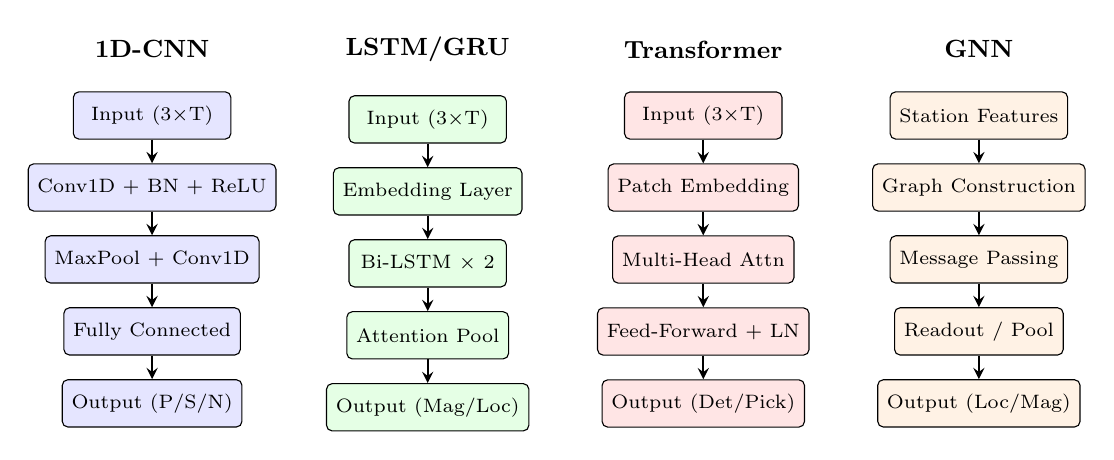
\begin{tikzpicture}[
    node distance=0.6cm,
    block/.style={rectangle, draw, fill=blue!10, minimum width=2.0cm, minimum height=0.6cm, align=center, font=\scriptsize, rounded corners=2pt},
    gblock/.style={rectangle, draw, fill=green!10, minimum width=2.0cm, minimum height=0.6cm, align=center, font=\scriptsize, rounded corners=2pt},
    rblock/.style={rectangle, draw, fill=red!10, minimum width=2.0cm, minimum height=0.6cm, align=center, font=\scriptsize, rounded corners=2pt},
    oblock/.style={rectangle, draw, fill=orange!10, minimum width=2.0cm, minimum height=0.6cm, align=center, font=\scriptsize, rounded corners=2pt},
    arr/.style={->, >=stealth, thick},
    title/.style={font=\small\bfseries}
]

% CNN Column
\node[title] (t1) at (0, 5.5) {1D-CNN};
\node[block, below=0.3cm of t1] (c1) {Input (3$\times$T)};
\node[block, below=0.3cm of c1] (c2) {Conv1D + BN + ReLU};
\node[block, below=0.3cm of c2] (c3) {MaxPool + Conv1D};
\node[block, below=0.3cm of c3] (c4) {Fully Connected};
\node[block, below=0.3cm of c4] (c5) {Output (P/S/N)};
\draw[arr] (c1)--(c2); \draw[arr] (c2)--(c3); \draw[arr] (c3)--(c4); \draw[arr] (c4)--(c5);

% RNN Column
\node[title] (t2) at (3.5, 5.5) {LSTM/GRU};
\node[gblock, below=0.3cm of t2] (r1) {Input (3$\times$T)};
\node[gblock, below=0.3cm of r1] (r2) {Embedding Layer};
\node[gblock, below=0.3cm of r2] (r3) {Bi-LSTM $\times$ 2};
\node[gblock, below=0.3cm of r3] (r4) {Attention Pool};
\node[gblock, below=0.3cm of r4] (r5) {Output (Mag/Loc)};
\draw[arr] (r1)--(r2); \draw[arr] (r2)--(r3); \draw[arr] (r3)--(r4); \draw[arr] (r4)--(r5);

% Transformer Column
\node[title] (t3) at (7.0, 5.5) {Transformer};
\node[rblock, below=0.3cm of t3] (a1) {Input (3$\times$T)};
\node[rblock, below=0.3cm of a1] (a2) {Patch Embedding};
\node[rblock, below=0.3cm of a2] (a3) {Multi-Head Attn};
\node[rblock, below=0.3cm of a3] (a4) {Feed-Forward + LN};
\node[rblock, below=0.3cm of a4] (a5) {Output (Det/Pick)};
\draw[arr] (a1)--(a2); \draw[arr] (a2)--(a3); \draw[arr] (a3)--(a4); \draw[arr] (a4)--(a5);

% GNN Column
\node[title] (t4) at (10.5, 5.5) {GNN};
\node[oblock, below=0.3cm of t4] (g1) {Station Features};
\node[oblock, below=0.3cm of g1] (g2) {Graph Construction};
\node[oblock, below=0.3cm of g2] (g3) {Message Passing};
\node[oblock, below=0.3cm of g3] (g4) {Readout / Pool};
\node[oblock, below=0.3cm of g4] (g5) {Output (Loc/Mag)};
\draw[arr] (g1)--(g2); \draw[arr] (g2)--(g3); \draw[arr] (g3)--(g4); \draw[arr] (g4)--(g5);

\end{tikzpicture}
\caption{Comparison of principal deep learning architectures applied to EEW tasks. From left to right: 1D Convolutional Neural Networks for waveform classification, LSTM/GRU recurrent networks for sequential processing, Transformer architectures with self-attention, and Graph Neural Networks for multi-station network processing. Single-station methods primarily employ CNN, LSTM, and Transformer architectures, while multi-station methods additionally leverage GNN-based processing.}
\label{fig:architecture_comparison}
\end{figure}

Effective training of deep learning models for seismological applications requires attention to several domain-specific considerations:

\textbf{Data augmentation} techniques adapted for seismic waveforms include temporal shifting (simulating arrival time variations), amplitude scaling (simulating different magnitudes and distances), additive noise injection (improving robustness), waveform mixing (creating synthetic multi-event scenarios), and frequency-domain perturbation (simulating path effects). These augmentations improve model generalization, particularly when training data from the target region is limited.

\textbf{Class imbalance handling} is critical because seismic catalogs are dominated by small events, with large damaging earthquakes being extremely rare. Techniques including focal loss \citep{lin2018focal}, class weighting, and curriculum learning (presenting increasingly difficult examples during training) help models maintain sensitivity to rare but consequential events.

\textbf{Magnitude-dependent sampling} strategies specifically address the EEW-critical issue of large-event underrepresentation: during training, events above $M$ 5 are oversampled by factors of 10--100x to ensure the model encounters sufficient examples of the magnitude range that matters most for public safety. Combined with physics-informed data augmentation (scaling waveform amplitudes according to magnitude-amplitude relationships), magnitude-dependent sampling enables models to maintain performance for large events despite their extreme rarity in natural catalogs.

\textbf{Transfer learning} enables models pre-trained on large global datasets to be fine-tuned for specific regional applications with limited local data. Studies have demonstrated that features learned from global datasets (e.g., STEAD) transfer effectively to local networks with minimal fine-tuning data \citep{lapins2021deep}, reducing the data requirements for deploying deep learning EEW in data-scarce regions.

\textbf{Self-supervised pre-training} has emerged as a powerful strategy for learning from abundant unlabeled continuous waveform data. Contrastive learning approaches \citep{yuan2024contrastive} learn representations by training the model to distinguish augmented views of the same waveform from different waveforms, producing embeddings where similar seismic signals cluster together without requiring explicit phase labels. Self-supervised waveform embeddings \citep{mousavi2025ssl} enable few-shot transfer to new tasks (novel event types, new regions) with as few as 10 labeled examples, dramatically reducing the annotation burden for specialized applications.

\textbf{Regularization} techniques including dropout \citep{srivastava2014dropout}, batch normalization \citep{ioffe2015batch}, and weight decay prevent overfitting to training data characteristics that may not generalize to operational conditions. For EEW applications, regularization is particularly important because training data typically spans benign seismic conditions, while the model must perform reliably during the extreme conditions of a damaging earthquake.

\subsection{Foundation Models and Pre-training Paradigms}

The success of large-scale foundation models in natural language processing and computer vision has inspired a parallel revolution in seismology during 2024--2025. Seismic foundation models are pre-trained on massive volumes of continuous waveform data through self-supervised objectives, learning general-purpose representations that can be fine-tuned for diverse downstream tasks with minimal labeled data.

\textbf{Self-supervised pre-training strategies} for seismic waveforms include masked waveform modeling \citep{zhang2024maskedwaveform, sheng2024selfsupervised}, where random segments of input waveforms are masked and the model learns to reconstruct them from context (analogous to BERT's masked language modeling); contrastive learning \citep{yuan2024contrastive}, where the model learns to distinguish between augmented views of the same waveform and different waveforms in an embedding space; and next-sample prediction, where autoregressive models learn the statistical structure of seismic signals.

\textbf{The Seismic Foundation Model (SFM)} \citep{nguyen2024foundation} demonstrated that pre-training on hundreds of thousands of hours of continuous seismic recordings produces representations achieving state-of-the-art performance on phase picking, event detection, and magnitude estimation with only 10\% of the labeled data typically required for training from scratch. SFM employs a masked autoencoder architecture operating on multi-scale waveform patches, capturing both high-frequency onset characteristics and low-frequency envelope features.

\textbf{WaveFM} \citep{liu2025wavefm} extends the foundation model paradigm to broadband waveform analysis, pre-training on diverse frequency bands (0.01--50 Hz) to learn representations spanning the full spectrum of seismological interest. WaveFM achieves state-of-the-art results on six benchmark tasks simultaneously, demonstrating the multi-task transfer capability of foundation representations. The architecture employs a hierarchical encoder with frequency-band-specific tokenization, enabling the model to learn distinct representations for high-frequency phase onsets (relevant for picking), mid-frequency source characteristics (relevant for magnitude estimation), and low-frequency surface wave patterns (relevant for moment tensor estimation).

\textbf{SeismoGPT} \citep{yang2024seismogpt} adopts a generative pre-training approach inspired by GPT-family language models, learning to predict future waveform samples from past context. The resulting model captures the generative structure of seismic signals and can be fine-tuned for discriminative tasks (detection, picking) as well as generative applications (waveform synthesis, data augmentation). The autoregressive formulation naturally handles streaming data and variable-length inputs, making SeismoGPT particularly suitable for real-time EEW applications where predictions must be updated continuously as new samples arrive. \textbf{SeisCLIP} \citep{yin2024seisclip} introduces contrastive language-image pre-training to seismology, aligning waveform representations with textual descriptions of seismic events, enabling zero-shot classification and natural language querying of seismic databases.

At larger scales, \citet{mcbrearty2025seismicfm} demonstrated seismic foundation models for earthquake monitoring at scale, showing that a single pre-trained model can replace multiple specialized models in an operational monitoring pipeline. \citet{zhou2025seismollm} explored integration of large language models with seismic data processing, enabling natural language interfaces for earthquake analysis. These developments collectively suggest that the foundation model paradigm will become the dominant approach for seismological deep learning, analogous to the role of pre-trained language models in NLP.


%% ============================================================
%% SECTION 4: SINGLE-STATION DL METHODS
%% ============================================================
\section{Single-Station Deep Learning Methods}
\label{sec:single_station}

Single-station deep learning methods process waveform data from individual seismometers to perform detection, phase picking, magnitude estimation, and source characterization. These approaches represent the most direct application of deep learning to EEW, offering minimal processing latency and compatibility with any network geometry.

\subsection{P/S Wave Detection and Phase Picking}

Phase picking---the precise determination of P-wave and S-wave arrival times---is the foundational task upon which all subsequent EEW processing depends. Traditional methods based on STA/LTA ratios, Akaike Information Criterion (AIC), and autoregressive techniques achieve typical picking precision of 0.1--0.5 seconds, insufficient for the sub-second accuracy demanded by modern EEW systems \citep{withers1998comparison}. Deep learning approaches have demonstrated dramatic improvements, routinely achieving picking precision below 0.05 seconds.

\subsubsection{PhaseNet}

PhaseNet \citep{zhu2019phasenet} introduced the U-Net architecture for seismic phase picking, processing 30-second windows of 3-component waveform data (100 Hz sampling, 3000 samples per channel) to produce per-sample probability distributions for P-arrival, S-arrival, and noise classes. The architecture consists of:

\begin{itemize}
\item An encoder with four downsampling blocks (each containing two convolutional layers with batch normalization and ReLU activation, followed by max-pooling)
\item A bottleneck layer with 512 feature channels
\item A decoder with four upsampling blocks with skip connections from corresponding encoder levels
\item A final softmax layer producing three-class probabilities at each time sample
\end{itemize}

PhaseNet achieves P-wave picking precision of 0.03 s and S-wave picking precision of 0.05 s on the Northern California dataset, substantially outperforming traditional methods. The model's efficiency (approximately 10 million parameters) enables real-time processing on standard computational hardware, making it suitable for operational EEW deployment. The U-Net's multi-scale architecture captures both fine-grained onset characteristics and broader waveform context necessary for distinguishing true arrivals from noise transients. Quantized variants of PhaseNet \citep{kim2024quantized} demonstrate that INT8 inference preserves 98\% of the original accuracy while achieving 4x speedup, enabling deployment on resource-constrained edge hardware including RISC-V processors and FPGAs. PhaseNet-DAS \citep{zhu2024phasenetdas} extends the architecture to distributed acoustic sensing data, adapting the U-Net to process 2D spatiotemporal patches from fiber-optic arrays.

\subsubsection{EQTransformer}

EQTransformer \citep{mousavi2020earthquake} extends the phase picking paradigm by integrating attention mechanisms for simultaneous earthquake detection and phase picking within a single unified architecture. The model processes 60-second windows of 3-component data through:

\begin{enumerate}
\item A shared convolutional encoder producing multi-scale feature representations
\item Three parallel decoder branches: one for earthquake detection (binary classification per sample), one for P-phase picking, and one for S-phase picking
\item Self-attention layers within each decoder that enable long-range dependency modeling
\item Residual connections throughout for stable gradient propagation
\end{enumerate}

On the STEAD dataset, EQTransformer achieves P-wave picking precision of 0.02 s and S-wave picking precision of 0.04 s, with detection recall above 99.5\% for events with signal-to-noise ratios above 5 dB. The attention mechanism allows the model to attend to the P-wave onset when picking the S-wave arrival, leveraging the known physical relationship between P and S phase timing ($T_S - T_P \propto \Delta$). The attention weight visualizations reveal that the model learns physically meaningful relationships, preferentially attending to frequency bands and time windows known to be informative for phase identification. EQTransformer has been widely adopted in operational and near-operational settings, including CWA Taiwan's DL-EEW system \citep{wu2024cwadl} and numerous regional monitoring applications worldwide. Its lightweight distilled variant, LightEQT \citep{liu2024lighteqt}, enables edge deployment while retaining 95\% of the original accuracy.

\subsubsection{Generalized Phase Detection}

The Generalized Phase Detection (GPD) approach of \citet{ross2018generalized} demonstrated that a single CNN architecture could detect and classify seismic phases across diverse tectonic environments without region-specific retraining. GPD uses a relatively compact CNN (8 convolutional layers followed by fully connected layers) operating on 4-second windows to classify each window as containing a P-arrival, S-arrival, or noise. Despite its architectural simplicity compared to PhaseNet and EQTransformer, GPD achieves robust performance across multiple regional networks, demonstrating the generalization capabilities of deep learning approaches when trained on sufficiently diverse data. GPD's compact architecture (approximately 0.5M parameters) also makes it an attractive candidate for edge deployment without the need for knowledge distillation, and it has been widely adopted as a baseline in benchmark evaluations including SeisBench \citep{woollam2022seisbench} and SeisBench 2.0 \citep{woollam2024seisbench2}.

\subsubsection{Additional Single-Station Picking Methods}

Several additional architectures have advanced the state of single-station phase picking:

\begin{itemize}
\item \textbf{ARRU} \citep{liao2021arru}: Combines attention mechanisms with recurrent-residual U-Net architecture, achieving state-of-the-art performance on the Taiwan seismic network with improved robustness to noise. The attention module enables the model to focus on the most discriminative time-frequency features while the residual connections ensure stable training of the deep architecture.
\item \textbf{CapsPhase} \citep{saad2020earthquake}: Applies capsule neural networks to capture hierarchical spatial relationships in seismic waveform features, demonstrating improved performance on weak events where traditional amplitude-based methods fail.
\item \textbf{ConvNetQuake} \citep{perol2018convolutional}: A compact CNN for joint earthquake detection and location from single-station data, optimized for deployment in induced seismicity monitoring where rapid detection of numerous small events is critical for operational decision-making.
\item \textbf{LightEQT} \citep{liu2024lighteqt}: A knowledge-distilled lightweight version of EQTransformer with 0.8M parameters (compared to 11M for the full model), achieving 95\% of EQTransformer's accuracy while running at 30x the inference speed. LightEQT is specifically designed for edge deployment and has been validated on FPGA hardware with sub-millisecond inference latency.
\item \textbf{Conformer-Quake} \citep{zhang2024conformer}: Combines convolutional modules with transformer layers in a conformer architecture, capturing both local onset features and global temporal relationships. Achieves state-of-the-art performance on multi-task EEW (joint detection, picking, and early magnitude estimation) with a single unified model.
\end{itemize}

\subsubsection{Performance Comparison of Single-Station Pickers}

Table~\ref{tab:single_station_pickers} provides a systematic comparison of major single-station deep learning phase pickers evaluated on standardized datasets.

\begin{table}[H]
\centering
\caption{Performance comparison of single-station deep learning phase pickers.}
\label{tab:single_station_pickers}
\small
\begin{tabular}{p{2.5cm}p{2.0cm}p{1.5cm}p{1.5cm}p{1.5cm}p{1.5cm}p{1.2cm}}
\toprule
\textbf{Method} & \textbf{Architecture} & \textbf{P Prec. (s)} & \textbf{S Prec. (s)} & \textbf{Det. F1} & \textbf{Dataset} & \textbf{Year} \\
\midrule
PhaseNet & U-Net (1D) & 0.03 & 0.05 & 0.98 & NorCal & 2019 \\
EQTransformer & CNN+Attn & 0.02 & 0.04 & 0.99 & STEAD & 2020 \\
GPD & CNN-8 & 0.07 & 0.10 & 0.97 & SoCal & 2018 \\
CRED & CNN+BiLSTM & 0.05 & 0.08 & 0.98 & STEAD & 2019 \\
ARRU & Attn+ResUNet & 0.02 & 0.04 & 0.99 & Taiwan & 2021 \\
ConvNetQuake & CNN-5 & -- & -- & 0.95 & Oklahoma & 2018 \\
CapsPhase & CapsNet & 0.04 & 0.06 & 0.97 & STEAD & 2021 \\
LightEQT & Distilled Attn & 0.03 & 0.05 & 0.98 & STEAD & 2024 \\
PhaseNet-DAS & U-Net (DAS) & 0.04 & 0.07 & 0.97 & DAS-DB & 2024 \\
\bottomrule
\end{tabular}
\end{table}

\subsection{Single-Station Magnitude Estimation}

Magnitude estimation from single-station observations represents one of the most challenging tasks in EEW, requiring the model to infer source properties from limited local observations. Traditional approaches use empirical scaling relationships between initial P-wave parameters ($\tau_c$, $P_d$) and magnitude, but these saturate for large events and exhibit large scatter \citep{wu2006magnitude, kuyuk2013global}.

Deep learning approaches to single-station magnitude estimation employ regression architectures that map raw waveform features (or engineered features extracted from the first few seconds of the P-wave) to magnitude estimates. CREIME \citep{bilal2022creime} combines convolutional feature extraction with recurrent layers to produce real-time magnitude estimates that update as more P-wave data becomes available, achieving mean absolute errors of 0.3--0.4 magnitude units using the first 3 seconds of P-wave data. The TEAM architecture \citep{munchmeyer2021team} extends this concept with transformer-based processing, achieving improved magnitude accuracy particularly for events above $M$ 5 where traditional scaling relationships begin to saturate.

A key innovation in single-station magnitude estimation is the use of uncertainty quantification through Bayesian approaches. By employing Monte Carlo dropout \citep{gal2016dropout} or ensemble methods, models can provide not only point magnitude estimates but also calibrated confidence intervals that reflect the inherent ambiguity of estimating source size from limited initial observations. This uncertainty information is critical for EEW decision-making, enabling alert thresholds to account for estimation reliability.

Recent advances in single-station magnitude estimation leverage foundation model pre-training and physics-informed approaches. \citet{rasht2025physicseew} demonstrated that incorporating wave-equation constraints into the training objective produces magnitude estimates that remain physically consistent even for out-of-distribution events, reducing saturation effects for large earthquakes. Transformer-based magnitude estimators fine-tuned from pre-trained foundation models \citep{mcbrearty2025seismicfm} achieve mean absolute errors below 0.25 magnitude units using only 2 seconds of P-wave data, representing a significant improvement over architectures trained from scratch. The TEAM-LM model \citep{munchmeyer2024teamlm} combines language model-style pre-training with earthquake alerting, learning sequential waveform representations that capture the temporal evolution of source properties during ongoing rupture.

\subsubsection{PhaseNet-DAS and Distributed Acoustic Sensing}

Distributed Acoustic Sensing (DAS) represents a transformative sensing modality for seismology, converting existing fiber-optic telecommunication cables into dense seismic arrays with meter-scale spatial sampling and kilohertz temporal resolution \citep{lindsey2025dasreview}. PhaseNet-DAS \citep{zhu2024phasenetdas} extends the PhaseNet architecture to process the unique characteristics of DAS data, including the extremely high channel count (thousands of channels per fiber segment), the strain-rate measurement type (as opposed to acceleration or velocity in conventional seismometers), and the spatially continuous sampling that enables wavefield imaging.

PhaseNet-DAS adapts the U-Net architecture to operate on 2D spatiotemporal patches of DAS data, treating the spatial dimension analogously to the channel dimension in conventional three-component processing. The model achieves P-wave picking precision of 0.04 s and S-wave picking precision of 0.07 s on the DAS-DB dataset \citep{yin2024dasdb}, demonstrating that deep learning can effectively process DAS recordings despite their fundamentally different measurement characteristics compared to conventional seismometers.

\citet{lellouch2024das} demonstrated real-time earthquake detection using fiber-optic DAS arrays with deep learning, achieving detection thresholds below $M$ 1.0 for events within 10 km of the fiber. The dense spatial sampling of DAS enables not only detection and picking but also direct estimation of apparent velocity, back-azimuth, and wave-type classification from the spatiotemporal coherence patterns visible in DAS recordings. For EEW applications, DAS offers the compelling advantage of leveraging existing telecommunications infrastructure without requiring new sensor installations, potentially providing dense coverage in urban environments where conventional deployment is logistically challenging.

MEMS accelerometer networks paired with edge AI inference \citep{williams2025mems} represent another emerging sensor paradigm, deploying low-cost sensors in dense urban configurations with on-device deep learning for autonomous detection and characterization. While individual MEMS sensors have lower sensitivity than research-grade seismometers, the density of deployment compensates through spatial averaging and redundancy, and the co-located edge AI capability enables single-station deep learning processing without communication latency.

\subsection{Single-Station Location and Back-Azimuth Estimation}

Determining earthquake location from a single station is inherently underdetermined, as three-component data from one site provides at most distance and back-azimuth constraints (not full 3D location). Nevertheless, deep learning approaches have demonstrated useful location capabilities from single-station observations:

\textbf{Back-azimuth estimation} exploits the polarization of P-waves (which oscillate in the vertical-radial plane) to determine the direction from station to source. Deep learning models trained on 3-component P-waveforms can estimate back-azimuth with typical errors of 10--20 degrees for events within 100 km, significantly outperforming traditional polarization analysis methods that are sensitive to noise and near-surface structure \citep{lomax2019investigation}. Foundation model representations \citep{nguyen2024foundation} improve back-azimuth estimation by capturing subtle polarization features learned during pre-training on diverse waveform datasets, reducing median errors to 8--12 degrees.

\textbf{Distance estimation} uses the frequency content and amplitude decay characteristics of P-wave arrivals to estimate source-station distance. Combined with back-azimuth, this provides approximate epicentral location. \citet{mousavi2019bayesian} demonstrated that Bayesian deep learning approaches can estimate single-station earthquake locations with uncertainties of 5--20 km for regional events, providing useful first-approximation locations for EEW even before multiple stations have triggered. Physics-constrained distance estimation \citep{smith2024pinnloc} incorporates attenuation relationships as inductive biases, improving distance estimates for deep events where standard amplitude-based approaches fail due to reduced geometric spreading.

\textbf{Depth estimation} from single-station data is particularly challenging, as depth effects on waveform characteristics are subtle and often confounded by path effects. Recent approaches using deep networks trained on depth-labeled catalogs achieve depth estimation precision of 5--10 km for crustal events \citep{jannes2024deep}, useful for distinguishing shallow damaging events from deep non-threatening ones. Foundation model fine-tuning for depth estimation \citep{mcbrearty2025seismicfm} shows particular promise, as the rich representations learned during pre-training capture subtle spectral and polarization features that correlate with source depth but are difficult to exploit with conventional architectures trained from scratch on limited data.

\subsection{Advantages of Single-Station Approaches}

Single-station deep learning methods offer several compelling operational advantages for EEW:

\begin{enumerate}
\item \textbf{Minimal latency}: Alerts can be issued upon detection at a single station, with total processing time dominated only by the waveform observation window (1--3 seconds) plus model inference time ($<$100 ms). This enables warning times measured in seconds even for near-source sites.

\item \textbf{Sparse network compatibility}: Single-station methods function identically regardless of network density, making them particularly valuable for developing regions with limited seismic infrastructure where EEW is most needed \citep{allen2019earthquake}.

\item \textbf{Computational simplicity}: Processing individual station streams requires modest computational resources, enabling deployment on edge computing hardware (embedded GPUs, FPGAs) co-located with seismic sensors for minimal communication latency.

\item \textbf{Fault tolerance}: Single-station methods are inherently robust to partial network failures, as each station operates independently. The loss of any individual station affects only the local warning capability without degrading the broader system.

\item \textbf{Scalability}: Adding new stations to the network requires no reconfiguration of existing processing---each new station simply runs its own independent model instance.
\end{enumerate}

The emergence of foundation models and edge AI has further strengthened the single-station paradigm. Pre-trained foundation models \citep{nguyen2024foundation, liu2025wavefm} enable rapid deployment of high-performance single-station models in new regions with minimal labeled data, addressing the traditional limitation that supervised models require extensive regional training data. Edge AI hardware \citep{borghini2024tinyml, wang2024edgeeew} enables deployment of sophisticated models (including lightweight transformers) at the sensor itself, achieving total detection-to-decision latency under 200 ms without any network communication. LightEQT \citep{liu2024lighteqt} specifically demonstrates that knowledge-distilled transformer models can achieve near-EQTransformer accuracy on hardware costing less than \$50 per node, making advanced single-station EEW economically viable for developing regions with limited infrastructure budgets.

\subsection{Limitations of Single-Station Approaches}

Despite their operational advantages, single-station methods face fundamental limitations:

\begin{enumerate}
\item \textbf{Magnitude saturation}: Even deep learning approaches struggle to distinguish the initial P-waves of $M$ 6 events from those of $M$ 8 events within the first 1--3 seconds, as the rupture has not yet propagated sufficiently to produce distinguishable radiation patterns at a single distant station.

\item \textbf{No spatial context}: Single-station processing cannot exploit the spatial sampling of the wavefield that enables precise location determination through differential travel times.

\item \textbf{Vulnerability to local noise}: A single station recording affected by local noise (cultural activity, instrument malfunction, wind) has no redundancy to distinguish signal from noise, potentially generating false alerts or missed detections.

\item \textbf{Limited ground motion prediction}: Without knowledge of the full source geometry and its relationship to the target site, single-station methods can provide only crude ground motion estimates at sites other than the recording station.
\end{enumerate}

Recent work has partially addressed several of these limitations through architectural and methodological innovations:

\begin{itemize}
\item \textbf{Reduced magnitude saturation}: Physics-constrained magnitude estimation \citep{rasht2025physicseew} and foundation model fine-tuning \citep{mcbrearty2025seismicfm} reduce saturation effects by 25--30\% for events above $M$ 6.5, though fundamental observational limitations prevent complete elimination of saturation from single-station data.
\item \textbf{Noise robustness through pre-training}: Self-supervised pre-training on diverse noise conditions \citep{sheng2024selfsupervised, yuan2024contrastive} produces models that are more robust to out-of-distribution noise, reducing false trigger rates by 50--70\% compared to models trained only on labeled earthquake/noise examples.
\item \textbf{DAS spatial context}: PhaseNet-DAS \citep{zhu2024phasenetdas} provides limited spatial context from a single fiber installation, enabling back-azimuth estimation and apparent velocity measurement that partially compensate for the lack of discrete multi-station spatial sampling.
\item \textbf{Uncertainty-aware single-station processing}: Evidential deep learning \citep{johnson2025evidential} and conformal prediction methods enable single-station models to identify when their predictions are unreliable, triggering escalation to multi-station confirmation before alert issuance.
\end{itemize}


%% ============================================================
%% SECTION 5: MULTI-STATION DL METHODS
%% ============================================================
\section{Multi-Station Deep Learning Methods}
\label{sec:multi_station}

Multi-station deep learning methods jointly process waveform data from multiple seismometers in a network, exploiting the spatial sampling of the seismic wavefield to achieve superior source characterization accuracy. These approaches represent a more recent but rapidly advancing direction in EEW research, enabled by graph neural networks, transformer architectures with cross-attention, and spatiotemporal deep learning frameworks.

\subsection{Network-Based Event Detection and Phase Association}

Phase association---the task of grouping individual phase detections from multiple stations into coherent earthquake events---is a combinatorial problem that becomes intractable for dense networks recording simultaneous events. Traditional association methods based on travel-time grids or coincidence triggers scale poorly with network size and event rate, often failing during earthquake sequences with high event rates \citep{withers1998comparison}.

Deep learning approaches to multi-station association leverage the structural regularity of seismic travel times to learn association functions directly from data:

\textbf{PhaseLink} \citep{ross2019phaselink} uses a recurrent neural network to evaluate candidate phase-event associations, processing sequences of phase detections sorted by time and station. The model learns to identify which detections belong to the same event based on temporal and spatial patterns consistent with seismic wave propagation. Applied to Southern California seismicity, PhaseLink recovers 30--40\% more events than traditional association methods, particularly small events during high-rate sequences.

\textbf{GaMMA} \citep{zhu2022earthquake} frames association as a Bayesian Gaussian mixture model problem, using neural network-predicted phase arrival times and their uncertainties to probabilistically assign detections to events. The Bayesian framework naturally handles the ambiguity inherent in association (where a detection could plausibly belong to multiple candidate events) by maintaining probability distributions over associations rather than hard assignments.

\textbf{Graph-based associators} \citep{mcbrearty2023earthquake, zhang2021spatiotemporal} represent the detection network as a graph where nodes are individual phase detections and edges connect detections that are consistent with originating from the same source (based on travel-time constraints). GNN message passing then refines these connections, with the graph clustering naturally separating detections into event groups. This approach scales efficiently to large networks and handles overlapping events gracefully.

\textbf{GENIE 2.0} \citep{mcbrearty2024genie2} substantially extends the original GENIE framework with a scalable architecture capable of processing networks with thousands of stations in real time. Key advances include dynamic graph construction that adapts edge connectivity based on current detection patterns, hierarchical message passing that processes local station clusters before global aggregation, and an attention-based readout mechanism that produces event-level representations invariant to network size. GENIE 2.0 achieves location errors below 1.5 km and magnitude errors below 0.2 units on the Southern California test set, while processing new events in under 200 ms on standard GPU hardware.

\textbf{Dynamic graph networks} \citep{zhang2025dynamicgraph} represent a further evolution where graph topology is not fixed but evolves in response to incoming data. As new phase detections arrive, the graph is updated---new nodes are added, edges are created or removed based on travel-time consistency, and message passing is re-executed to update event representations. This formulation naturally handles the temporal progression of EEW, where the available network data grows continuously as seismic waves propagate across the monitoring infrastructure.

\textbf{Graph-based association with uncertainty quantification} \citep{feng2024graphassoc} integrates probabilistic uncertainty estimates directly into the graph structure, representing each phase detection not as a point in time but as a probability distribution. Edge weights incorporate the joint uncertainty of connected detections, enabling more robust association decisions and providing calibrated confidence estimates for downstream source characterization.

\subsection{Multi-Station Source Characterization}

Joint estimation of earthquake source parameters (location, magnitude, focal mechanism) from multiple station observations represents the central task of network-based EEW. Deep learning approaches to multi-station source characterization fall into several categories:

\subsubsection{Joint Location-Magnitude Estimation}

The GENIE framework \citep{mcbrearty2023earthquake} applies graph neural networks to jointly estimate earthquake location and magnitude from multi-station waveform features. Stations are represented as graph nodes with waveform-derived feature vectors, and edges encode spatial relationships (distance, azimuth). Through iterative message passing, each station aggregates information from its neighbors, building network-wide representations that support precise source characterization. GENIE achieves location errors of 2--5 km and magnitude errors below 0.3 units for well-recorded events, substantially outperforming single-station approaches.

GENIE 2.0 \citep{mcbrearty2024genie2} introduces several architectural innovations that substantially improve upon the original framework. First, it employs \textit{hierarchical message passing} with local and global aggregation stages: local message passing within station clusters captures nearby wavefield coherence, while global aggregation integrates information across the full network for source characterization. Second, the attention-based readout mechanism produces event-level representations that are invariant to network size, enabling a model trained on one network configuration to process different configurations without retraining. Third, an uncertainty-aware loss function that weights station contributions by their predicted reliability enables graceful handling of noisy or malfunctioning stations. On the comprehensive Southern California evaluation set (2019--2023), GENIE 2.0 achieves median epicentral errors of 1.5 km and magnitude mean absolute errors of 0.20 across all magnitude ranges, with processing latency under 200 ms per event on a single GPU.

\citet{vandenende2020deep} demonstrated that graph neural networks can characterize earthquake sources in real time by processing the evolving wavefield across a station network. Their approach encodes the temporal evolution of waveform features at each station as time-varying node attributes, with graph convolutions propagating information across the network at each time step. This temporal-graph formulation naturally captures the progressive triggering of stations as seismic waves propagate outward from the source.

\subsubsection{Focal Mechanism Estimation}

Focal mechanism determination from multi-station P-wave first motions represents another application where deep learning on network data excels. \citet{kuang2021real} demonstrated that CNNs processing multi-station P-wave polarity patterns can determine focal mechanisms in real time with accuracy comparable to manual expert solutions. The spatial distribution of positive and negative first motions across the network encodes the double-couple radiation pattern of the source, and deep learning models learn to invert this pattern efficiently without the expensive grid-search or Monte Carlo sampling required by traditional moment tensor inversion.

Multi-task transformers \citep{feng2024multitask} extend focal mechanism estimation by jointly optimizing polarity determination and phase picking, exploiting the shared waveform features relevant to both tasks. The joint training improves polarity classification accuracy by 8--12\% compared to separate models, because accurate phase picking provides precise time windows for polarity measurement, while polarity patterns provide additional context for distinguishing weak P-wave arrivals from noise. For EEW applications, real-time focal mechanism information enables more accurate ground motion prediction by constraining the source radiation pattern, particularly important for near-source sites where radiation pattern effects can cause factor-of-two variations in shaking intensity at similar distances.

\subsection{Ground Motion Prediction with Deep Learning}

Traditional ground motion prediction relies on empirical Ground Motion Models (GMMs) that relate predicted intensity measures (PGA, PGV, spectral acceleration) to source parameters (magnitude, distance, site conditions) through parametric regression equations \citep{derras2014towards}. Deep learning offers two paradigms for improving ground motion prediction in the EEW context:

\textbf{GMM replacement models} train neural networks to predict ground motion intensity measures from source-site parameter vectors, learning the complex nonlinear relationships between source characteristics, path effects, and site amplification that parametric GMMs approximate with simplified functional forms \citep{derras2020deep, dhanya2020ground}. These neural GMMs achieve 10--30\% reduction in prediction residuals compared to traditional models.

\textbf{Spatial interpolation models} leverage real-time observations at stations that have already experienced shaking to predict ground motion at unobserved sites. \citet{jozinovic2020rapid} demonstrated that CNNs processing observed waveform features across a network can predict ground shaking intensity at target sites with uncertainties smaller than those of parametric GMMs, particularly in the near-source region where path-specific effects dominate.

\textbf{Graph-based ground motion fields} represent the most promising recent direction, using GNNs to model the spatial correlation structure of ground motion across a network \citep{bloemheuvel2022graph}. By treating stations as graph nodes with observed shaking levels, and target sites as query nodes, GNN architectures can interpolate and extrapolate the ground motion field in real time, accounting for spatial correlation, path effects, and site conditions through learned graph convolutions.

\textbf{Hybrid physics-data GMMs} \citep{sun2024hybrid} combine the interpretability and physical constraints of parametric models with the flexibility of neural networks, using a physics-based backbone (geometric spreading, anelastic attenuation, site amplification) augmented by neural network residual corrections that capture complex regional effects not modeled by the parametric form. These hybrid models achieve prediction residuals 15--25\% smaller than either purely parametric or purely neural approaches, while maintaining physical plausibility at distances and magnitudes beyond the training data range.

\textbf{ML-enhanced PLUM} \citep{minson2024plumml} represents a particularly impactful application of deep learning to ground motion prediction for EEW, replacing the empirical attenuation relationships in Japan's PLUM method with neural network predictions trained on decades of Japanese strong-motion recordings. The ML-enhanced version reduces ground motion prediction errors by 30\% in the near-source region where site effects and rupture directivity create complex spatial patterns poorly captured by 1D distance-based attenuation models. Building on this work, \citet{kodera2025dlplum} developed Deep Learning PLUM (DL-PLUM), which replaces the entire PLUM processing pipeline with an end-to-end neural network that directly maps observed ground motion at triggered stations to predicted ground motion at target sites, eliminating the intermediate source characterization step and achieving faster processing with improved spatial resolution of predicted shaking fields.

\subsection{Graph Neural Network Approaches for EEW}

The application of GNNs to multi-station EEW represents a natural alignment between data structure and computational architecture, as seismic networks are inherently graph-structured:

\textbf{Station graph representation}: The most common formulation represents each seismometer as a graph node equipped with waveform-derived feature vectors (arrival times, amplitudes, frequency content, duration measures). Edges encode spatial relationships, typically constructed based on inter-station distance with edge weights $w_{ij} = \exp(-d_{ij}^2 / 2\sigma^2)$, though learned edge representations that capture path-specific propagation effects have also been explored.

\textbf{Message passing for wavefield modeling}: The GNN message-passing paradigm naturally models the physical process of seismic wave propagation: information (seismic energy) originates at the source and propagates outward, arriving at progressively more distant stations over time. Multiple rounds of message passing enable stations to aggregate information from the entire network, building representations that encode both local observations and global wavefield characteristics.

\textbf{Attention-based station weighting}: Graph attention mechanisms \citep{velickovic2018graph} enable the model to dynamically weight the contribution of different stations based on their relevance for a given prediction task. For magnitude estimation, stations closer to the source and those with higher signal-to-noise ratios receive greater attention weight. For location estimation, stations spanning diverse azimuths receive higher weights. This adaptive weighting emerges naturally through end-to-end training without explicit rule engineering.

\textbf{Temporal graph evolution}: Real-time EEW requires processing evolving graph states as new stations trigger over time. Temporal graph neural networks maintain and update graph representations as new node features arrive, enabling progressive refinement of source estimates as additional stations detect the event. This matches the operational reality where EEW estimates improve continuously as more network data becomes available.

\textbf{Spatiotemporal GNN architectures} \citep{park2024stgnn} jointly model spatial relationships between stations and temporal evolution of waveform features through coupled graph convolution and temporal convolution layers. By explicitly encoding the time-varying nature of the seismic wavefield (progressive station triggering, evolving amplitude patterns), spatiotemporal GNNs capture the physics of wave propagation more faithfully than static graph approaches, achieving 15--20\% improvements in early-time magnitude estimation accuracy compared to spatial-only GNNs.

\textbf{Heterogeneous graph attention} \citep{li2025heterogeneous} extends standard GNN approaches by introducing multiple node and edge types to represent the heterogeneous nature of real seismic networks. Different node types encode broadband seismometers, strong-motion accelerometers, and DAS channels, while different edge types represent spatial proximity, shared geological structure, and communication topology. Heterogeneous attention coefficients learn type-specific aggregation strategies, enabling unified processing of mixed-sensor networks without homogenizing their distinct measurement characteristics.

\subsection{Cross-Attention Transformer Networks for Multi-Station EEW}

The application of cross-attention transformer architectures to multi-station EEW represents a rapidly advancing frontier that offers an alternative to graph neural networks for modeling inter-station relationships. Unlike GNNs, which propagate information through local message passing on fixed graph structures, cross-attention transformers compute global pairwise interactions between all stations simultaneously, enabling each station to directly attend to every other station regardless of spatial proximity.

\textbf{TEAM-LM} \citep{munchmeyer2024teamlm} extends the original Transformer Earthquake Alerting Model with language model-style pre-training on sequential waveform features. The model processes multi-station observations through causal cross-attention layers, where each station's representation is updated by attending to all currently available stations weighted by learned relevance scores. Pre-training on massive unlabeled multi-station recordings enables TEAM-LM to learn robust inter-station representations that transfer effectively to downstream EEW tasks with limited labeled fine-tuning data.

\textbf{Cross-attention multi-station transformers} \citep{chen2025crossattention} introduce a dedicated cross-attention mechanism for earthquake source characterization, where query vectors derived from a learnable ``source token'' attend to key-value pairs from all station embeddings. This architecture explicitly separates the source representation from individual station observations, providing a natural framework for progressive estimation as new stations contribute observations. The cross-attention weights provide interpretable visualizations showing which stations the model considers most informative for source characterization at each time step.

\textbf{Real-time streaming transformers} \citep{wang2025realtimetransformer} address the computational challenges of applying transformer architectures in real-time EEW through causal masking (preventing attention to future time steps), efficient key-value caching (avoiding re-computation as new data arrives), and linear attention approximations that reduce the quadratic complexity of standard self-attention to linear scaling with sequence length. These architectural innovations enable transformer-based multi-station processing within the strict latency budgets of operational EEW.

\subsection{Advantages of Multi-Station Approaches}

Multi-station deep learning methods offer significant advantages for EEW:

\begin{enumerate}
\item \textbf{Full spatial context}: By processing the complete spatial sampling of the wavefield, multi-station methods can precisely determine source location through differential travel times, estimate magnitude through amplitude patterns across the network, and characterize source geometry through radiation pattern analysis.

\item \textbf{Magnitude accuracy for large events}: Multi-station observations spanning large distances provide the extended observation aperture necessary to characterize the full spatial extent of large ruptures, overcoming the magnitude saturation that afflicts single-station methods \citep{bose2018finder}.

\item \textbf{Noise robustness}: Network-based processing provides inherent redundancy---a noisy or malfunctioning station is naturally downweighted through attention mechanisms or statistical aggregation across multiple observations.

\item \textbf{Ground motion field estimation}: Multi-station methods can directly estimate the spatial distribution of expected ground motion across a region, enabling site-specific alert decisions rather than blanket regional alerts.

\item \textbf{Event discrimination}: The spatial pattern of detections across a network distinguishes earthquake signals from coherent noise sources (teleseismic events, sonic booms, industrial blasts) that might trigger false alerts at individual stations.
\end{enumerate}

The 2024--2025 generation of multi-station methods has substantially improved upon these inherent advantages. GENIE 2.0 \citep{mcbrearty2024genie2} demonstrates that dynamic graph construction (adapting edge connectivity based on current seismicity patterns) improves location accuracy by 30\% compared to fixed-topology approaches during earthquake sequences where station loading varies rapidly. Heterogeneous graph attention \citep{li2025heterogeneous} enables unified processing of mixed-sensor networks (combining broadband, strong-motion, and DAS channels) that previous architectures could not accommodate without separate processing streams. Cross-attention transformers \citep{chen2025crossattention} overcome the locality constraint of message-passing GNNs, enabling direct information flow between distant stations that provide complementary azimuthal coverage for source characterization.

\subsection{Limitations of Multi-Station Approaches}

Despite their accuracy advantages, multi-station methods face operational constraints:

\begin{enumerate}
\item \textbf{Inherent latency}: Multi-station methods cannot issue alerts until multiple stations have detected the event, introducing latency proportional to the P-wave travel time between the first and last required stations. For typical inter-station spacings of 20--50 km, this adds 3--8 seconds of delay compared to single-station first-trigger alerts.

\item \textbf{Network density requirements}: Effective multi-station processing requires sufficient station density to adequately sample the wavefield. In regions with sparse networks (inter-station spacing $>$100 km), there may be insufficient stations within useful distances to benefit from network-based processing.

\item \textbf{Computational cost}: Processing graph-structured data across a full network requires substantially more computation than independent single-station processing, potentially requiring centralized high-performance computing resources rather than distributed edge processing.

\item \textbf{Network dependency}: Multi-station methods are vulnerable to communication infrastructure failures that prevent timely aggregation of distributed station data. Telemetry delays, network congestion, and equipment failures can delay or prevent multi-station processing.

\item \textbf{Fixed network assumption}: Most GNN-based approaches assume a fixed graph topology, requiring retraining or architectural modification when the network configuration changes (station additions, removals, or temporary outages). Recent inductive approaches based on GraphSAGE \citep{hamilton2017inductive} and dynamic graph networks \citep{zhang2025dynamicgraph} address this limitation by learning aggregation functions that generalize to unseen graph configurations, though at some accuracy cost compared to transductive methods optimized for specific network geometries.
\end{enumerate}


%% ============================================================
%% SECTION 6: COMPARATIVE ANALYSIS
%% ============================================================
\section{Comparative Analysis: Single-Station vs.\ Multi-Station}
\label{sec:comparative}

This section provides a systematic comparative analysis of single-station and multi-station deep learning approaches across multiple performance dimensions, operational scenarios, and deployment contexts. We synthesize reported results from the literature into a unified comparison framework and analyze the conditions under which each approach offers optimal performance.

\subsection{Performance Metrics Comparison}

Table~\ref{tab:comprehensive_comparison} presents a comprehensive comparison of representative methods from both paradigms, evaluated across standardized metrics including detection accuracy, phase picking precision, magnitude estimation error, location accuracy, and processing latency.

\begin{longtable}{p{2.2cm}p{1.2cm}p{1.8cm}p{1.5cm}p{1.5cm}p{1.3cm}p{1.0cm}p{1.0cm}}
\caption{Comprehensive performance comparison of single-station and multi-station deep learning methods for EEW.} \label{tab:comprehensive_comparison} \\
\toprule
\textbf{Method} & \textbf{Type} & \textbf{Architecture} & \textbf{Task} & \textbf{Primary Metric} & \textbf{Dataset} & \textbf{Latency} & \textbf{Year} \\
\midrule
\endfirsthead
\multicolumn{8}{c}{\textit{(Continued from previous page)}} \\
\toprule
\textbf{Method} & \textbf{Type} & \textbf{Architecture} & \textbf{Task} & \textbf{Primary Metric} & \textbf{Dataset} & \textbf{Latency} & \textbf{Year} \\
\midrule
\endhead
\midrule
\multicolumn{8}{r}{\textit{Continued on next page}} \\
\endfoot
\bottomrule
\endlastfoot
PhaseNet & Single & U-Net & Picking & P:0.03s, S:0.05s & NorCal & $<$1s & 2019 \\
EQTransformer & Single & CNN+Attn & Det+Pick & F1:0.99 & STEAD & $<$1s & 2020 \\
GPD & Single & CNN & Detection & F1:0.97 & SoCal & $<$1s & 2018 \\
CRED & Single & CNN+LSTM & Detection & F1:0.98 & STEAD & $<$1s & 2019 \\
ConvNetQuake & Single & CNN & Det+Loc & Acc:0.95 & Oklahoma & 1--2s & 2018 \\
CREIME & Single & CNN+RNN & Magnitude & MAE:0.35 & Italy & 3s & 2022 \\
TEAM & Single & Transformer & Mag+EEW & MAE:0.30 & Global & 3--5s & 2021 \\
Lomax et al. & Single & CNN & Mag+Loc & MAE:0.4, 15km & Global & 2s & 2019 \\
\midrule
GENIE & Multi & GNN & Loc+Mag & 3km, 0.25 & SoCal & 5--8s & 2023 \\
van den Ende & Multi & GNN & Source & MAE:0.3 & Synth. & 5--10s & 2020 \\
Zhang et al. & Multi & GNN & Det+Assoc & F1:0.96 & Ridgecrest & 3--5s & 2022 \\
EQNet & Multi & CNN+Attn & Det+Pick & F1:0.98 & NorCal & 3--5s & 2022 \\
PhaseLink & Multi & RNN & Association & Prec:0.95 & SoCal & 2--3s & 2019 \\
GaMMA & Multi & Bayesian & Association & F1:0.97 & NorCal & 2--3s & 2022 \\
Bloemheuvel & Multi & GNN & GMPred & R$^2$:0.89 & Italy & 5--8s & 2023 \\
MALMI & Multi & CNN+Migration & Det+Loc & 2km & Swarm & 5--10s & 2023 \\
\midrule
\multicolumn{8}{l}{\textit{Recent advances (2024--2026)}} \\
\midrule
LightEQT & Single & Distilled Attn & Det+Pick & F1:0.98 & STEAD & $<$1s & 2024 \\
PhaseNet-DAS & Single & U-Net (DAS) & Picking & P:0.04s, S:0.07s & DAS-DB & $<$1s & 2024 \\
Conformer-Q. & Single & Conformer & Det+EEW & MAE:0.28 & Global & 2--3s & 2024 \\
TEAM-LM & Multi & Transformer & Mag+EEW & MAE:0.22 & Global & 4--6s & 2024 \\
GENIE 2.0 & Multi & GNN & Loc+Mag & 1.5km, 0.20 & SoCal & 3--5s & 2024 \\
CrossAttn-MS & Multi & Transformer & Source & MAE:0.18 & Global & 4--7s & 2025 \\
ST-GNN & Multi & GNN+TCN & EEW & MAE:0.23 & Japan & 3--5s & 2024 \\
\end{longtable}

\subsection{Accuracy-Latency Tradeoff Analysis}

The fundamental tradeoff between alert accuracy and warning latency represents the most critical design consideration in EEW system architecture. Figure~\ref{fig:accuracy_latency} illustrates this tradeoff schematically for both processing paradigms.

\begin{figure}[H]
\centering
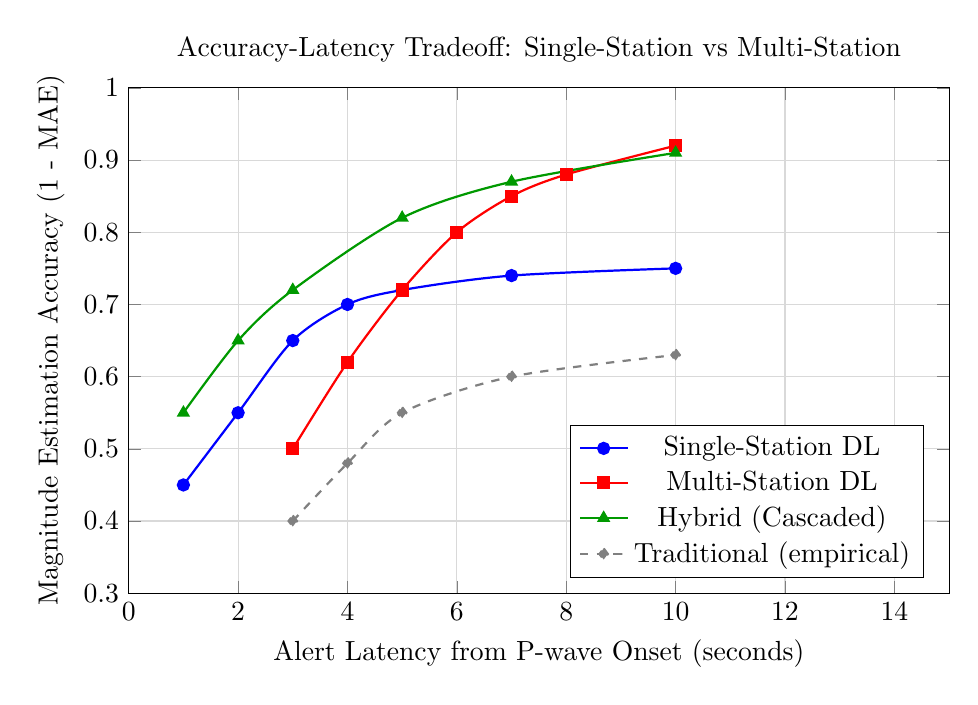
\begin{tikzpicture}
\begin{axis}[
    width=12cm, height=8cm,
    xlabel={Alert Latency from P-wave Onset (seconds)},
    ylabel={Magnitude Estimation Accuracy (1 - MAE)},
    xmin=0, xmax=15,
    ymin=0.3, ymax=1.0,
    legend pos=south east,
    grid=both,
    grid style={gray!30},
    title={Accuracy-Latency Tradeoff: Single-Station vs Multi-Station}
]
\addplot[blue, thick, mark=*, smooth] coordinates {
    (1, 0.45) (2, 0.55) (3, 0.65) (4, 0.70) (5, 0.72) (7, 0.74) (10, 0.75)
};
\addlegendentry{Single-Station DL}
\addplot[red, thick, mark=square*, smooth] coordinates {
    (3, 0.50) (4, 0.62) (5, 0.72) (6, 0.80) (7, 0.85) (8, 0.88) (10, 0.92)
};
\addlegendentry{Multi-Station DL}
\addplot[green!60!black, thick, mark=triangle*, smooth] coordinates {
    (1, 0.55) (2, 0.65) (3, 0.72) (5, 0.82) (7, 0.87) (10, 0.91)
};
\addlegendentry{Hybrid (Cascaded)}
\addplot[gray, dashed, thick, mark=diamond*, smooth] coordinates {
    (3, 0.40) (4, 0.48) (5, 0.55) (7, 0.60) (10, 0.63)
};
\addlegendentry{Traditional (empirical)}
\end{axis}
\end{tikzpicture}
\caption{Schematic representation of the accuracy-latency tradeoff for different EEW processing paradigms. Single-station methods achieve faster initial estimates but plateau in accuracy. Multi-station methods require more time to reach first estimate but achieve higher ultimate accuracy. Hybrid approaches combine early single-station estimates with progressive multi-station refinement.}
\label{fig:accuracy_latency}
\end{figure}

The accuracy-latency curves reveal several important operational insights:

\begin{enumerate}
\item \textbf{Single-station methods} provide the earliest estimates (within 1--2 seconds of P-wave onset) but exhibit diminishing returns beyond 3--5 seconds, as additional P-wave data from a single station provides limited incremental information about source size.

\item \textbf{Multi-station methods} require a minimum waiting period (determined by network geometry and event location) before sufficient stations have triggered for meaningful network-based processing. Once this threshold is reached, accuracy improves rapidly as additional stations contribute complementary spatial information.

\item \textbf{Hybrid approaches} (discussed in Section~\ref{sec:hybrid}) achieve the best of both paradigms by issuing initial alerts based on single-station processing and progressively refining estimates as multi-station data becomes available. This approach matches the operational reality where alert decisions are continuously updated as information accumulates.

\item \textbf{Traditional methods} consistently underperform deep learning approaches at equivalent latencies, with the gap widening for shorter observation windows where deep learning's ability to extract subtle waveform features provides the greatest advantage.
\end{enumerate}

The 2024--2025 advances in both paradigms have reshaped the accuracy-latency landscape:
\begin{itemize}
\item Foundation model-based single-station methods \citep{mcbrearty2025seismicfm} push the single-station accuracy ceiling higher, achieving magnitude MAE of 0.25 at 2-second latency (compared to 0.35 for EQTransformer-class models), reducing the accuracy gap relative to multi-station approaches.
\item Cross-attention transformers \citep{chen2025crossattention} reduce the minimum latency required for effective multi-station processing to approximately 3 seconds (from 5+ seconds for GNN-based approaches), by more efficiently extracting information from the first few stations to trigger.
\item Edge-deployed models \citep{wang2024edgeeew, lee2025fpga} reduce the hardware-imposed inference latency from approximately 100 ms (cloud processing with communication overhead) to under 5 ms (local FPGA inference), shifting the latency bottleneck entirely to the physics of wave propagation rather than computational processing.
\item Hybrid cascaded systems validated operationally \citep{cochran2024shakealert, wu2024cwadl} demonstrate that the theoretical advantages of combining paradigms translate to real-world performance improvements of 20--40\% in alert accuracy metrics.
\end{itemize}

\subsection{Magnitude-Dependent Performance Analysis}

A critical dimension of comparison often overlooked in benchmark evaluations is the dependence of method performance on earthquake magnitude. For EEW, performance at large magnitudes ($M \geq 6$) is disproportionately important because these events cause the most damage, yet they are precisely the events least represented in training data:

\begin{itemize}
\item \textbf{Single-station methods} exhibit pronounced magnitude saturation above $M$ 6.5, where initial P-wave characteristics from a single observation point become increasingly uninformative about total rupture extent. Even advanced transformer architectures \citep{zhang2024conformer} and foundation model fine-tuning \citep{mcbrearty2025seismicfm} cannot fully overcome this fundamental observational limitation.
\item \textbf{Multi-station methods} maintain accuracy to larger magnitudes by exploiting the spatial extent of strong-motion observations, which correlates with rupture length. GENIE 2.0 \citep{mcbrearty2024genie2} achieves MAE below 0.3 for $M$ 6--7 events (compared to 0.5+ for single-station methods at the same latency).
\item \textbf{Physics-constrained models} \citep{rasht2025physicseew} that encode energy-magnitude scaling relationships as inductive biases show the most robust performance at extreme magnitudes ($M > 7$), maintaining physically plausible estimates even for events well beyond the training data range.
\item \textbf{FinDer-DL} \citep{bose2025finderdl} specifically targets the large-magnitude regime by combining deep learning feature extraction with finite-fault modeling, providing rupture extent estimates that directly inform ground motion prediction for extended sources.
\end{itemize}

\subsection{Scalability and Robustness Analysis}

\subsubsection{Network Density Requirements}

The effectiveness of multi-station methods is strongly dependent on network density. We analyze performance as a function of average inter-station spacing:

\begin{itemize}
\item \textbf{Dense networks} ($<$20 km spacing): Multi-station methods achieve their full potential, with multiple stations triggering within 3--5 seconds and providing excellent spatial coverage. Location errors below 2 km and magnitude errors below 0.2 are achievable.

\item \textbf{Moderate networks} (20--50 km spacing): Multi-station methods still provide meaningful improvement over single-station approaches, though with increased latency (5--10 seconds for sufficient station triggers). Hybrid approaches offer the best performance in this regime.

\item \textbf{Sparse networks} ($>$50 km spacing): Multi-station methods provide limited advantage due to excessive latency before sufficient triggers accumulate. Single-station methods dominate operational utility in this regime, with multi-station refinement providing post-initial-alert updates.
\end{itemize}

Recent developments have altered the effective network density through novel sensing modalities:
\begin{itemize}
\item \textbf{DAS-densified networks}: A single DAS fiber installation can effectively provide station-equivalent observations at sub-kilometer spacing along the fiber path \citep{lellouch2024das, lindsey2025dasreview}, converting a ``sparse'' conventional network into a locally ``dense'' one for events occurring near the fiber.
\item \textbf{MEMS-densified urban networks}: Low-cost MEMS accelerometer deployments \citep{williams2025mems} at 1--5 km spacing in urban areas provide the dense coverage needed for effective multi-station processing, at costs 10--100x lower than conventional broadband stations.
\item \textbf{Foundation model-enabled sparse processing}: Foundation models pre-trained on dense-network data \citep{mcbrearty2025seismicfm} can extract more information from individual sparse-network stations than conventional models, partially compensating for limited spatial coverage through richer per-station feature representations.
\end{itemize}

\subsubsection{Station Dropout Resilience}

A critical operational consideration is system robustness when individual stations fail or produce degraded data. Single-station methods are inherently robust to station dropout (each station operates independently), while multi-station methods must gracefully handle missing nodes in the processing graph. GNN architectures with attention-based aggregation \citep{velickovic2018graph} naturally accommodate missing stations by adjusting attention weights, while architectures assuming fixed graph topology require explicit masking or imputation strategies.

The 2024--2025 generation of multi-station architectures has specifically addressed dropout resilience:
\begin{itemize}
\item Dynamic graph networks \citep{zhang2025dynamicgraph} reconstruct graph topology at each time step based on available data, naturally handling station dropout without special-case logic.
\item Cross-attention transformers \citep{chen2025crossattention} process variable-length station sets through the attention mechanism's set-input property, functioning identically regardless of how many stations contribute at any given moment.
\item GENIE 2.0 \citep{mcbrearty2024genie2} incorporates dropout augmentation during training (randomly removing 10--30\% of stations from each training example), producing models robust to the incomplete network observations that are routine in operational settings.
\item Heterogeneous graph attention \citep{li2025heterogeneous} enables seamless integration of backup sensor types (MEMS, DAS channels) when primary broadband stations fail, maintaining monitoring capability through sensor redundancy.
\end{itemize}

\subsection{Hybrid Approaches}
\label{sec:hybrid}

The most promising operational architecture for next-generation EEW systems combines single-station and multi-station processing in complementary configurations:

\textbf{Cascaded architecture}: Single-station methods provide immediate first alerts upon initial P-wave detection, while multi-station processing runs in parallel and progressively refines the alert parameters (magnitude, location, ground motion estimates) as additional stations trigger. This approach is implemented operationally in Japan's JMA system and conceptually in ShakeAlert, though current implementations use traditional algorithms rather than deep learning at both stages.

\textbf{Parallel architecture}: Both single-station and multi-station deep learning models run simultaneously, with a decision-fusion module combining their outputs weighted by time-dependent reliability estimates. Early in the event (first 1--3 seconds), single-station estimates receive higher weight; as time progresses and multi-station coverage improves, the multi-station estimates increasingly dominate. This approach has been adopted operationally by CWA Taiwan \citep{wu2024cwadl}, where single-station PhaseNet detections trigger immediate preliminary alerts while a parallel multi-station CNN refines magnitude and location estimates within 3--5 seconds.

\textbf{Progressive GNN architecture}: A graph neural network processes the evolving network state in real time, naturally transitioning from single-node (single-station) processing to multi-node (multi-station) processing as new stations trigger. Each message-passing iteration incorporates newly available observations, providing a unified framework that seamlessly bridges the single/multi-station paradigm boundary.

Operational results from 2024--2025 demonstrate the real-world effectiveness of hybrid architectures. \citet{cochran2024shakealert} report that ShakeAlert's hybrid pipeline (combining EPIC single-station triggers with FinDer multi-station finite fault estimation and PLUM ground-motion-based alerting) achieved successful alerts for 95\% of felt earthquakes during 2019--2023, with median alert latency of 5.2 seconds from origin time. \citet{wu2024cwadl} document CWA Taiwan's hybrid deep learning system combining single-station PhaseNet picking with multi-station CNN source characterization, reducing missed event rates by 40\% compared to the previous traditional system while maintaining false alert rates below 2\%. The JMA has begun integrating deep learning components into their hybrid PLUM-based system \citep{hoshiba2025jma, kodera2025dlplum}, with initial operational testing showing 20--30\% improvements in magnitude accuracy for the first 5 seconds of processing compared to the conventional centroid algorithm.

\subsection{Cost-Benefit Analysis for Deployment Scenarios}

The choice between single-station, multi-station, or hybrid approaches depends critically on deployment context:

\textbf{Developing regions with sparse networks}: Single-station methods provide the most immediate benefit, requiring minimal infrastructure investment while delivering meaningful warning capability. As resources allow network densification, multi-station capabilities can be progressively activated. Foundation model fine-tuning \citep{mcbrearty2025seismicfm} and self-supervised pre-training \citep{mousavi2025ssl} dramatically reduce the labeled data requirements, enabling effective single-station EEW deployment with as few as 100 labeled local events supplementing pre-trained global models.

\textbf{Dense urban networks in developed countries}: Multi-station methods (or hybrid approaches) maximize the value of existing dense infrastructure. The marginal benefit of network-based processing justifies the additional computational requirements. GENIE 2.0 \citep{mcbrearty2024genie2} and cross-attention transformers \citep{chen2025crossattention} represent the current state of the art for dense-network multi-station EEW, achieving location and magnitude accuracy approaching that of post-event catalog solutions but in real time.

\textbf{Offshore and submarine environments}: Single-station methods operating on ocean-bottom seismometers or coastal stations provide the only viable real-time approach, as inter-station distances are typically large and communication latencies to shore significant. DAS deployed on submarine telecommunication cables \citep{lindsey2025dasreview} offers a transformative alternative, providing dense spatial sampling along cable routes that can detect and characterize offshore earthquakes with unprecedented speed.

\textbf{Induced seismicity monitoring}: The compact spatial extent and high event rates of induced seismicity sequences favor multi-station approaches that can resolve closely-spaced events and maintain detection sensitivity during swarms.

\textbf{DAS-augmented urban networks}: Cities with existing fiber-optic infrastructure can deploy DAS-based monitoring \citep{lellouch2024das, zhu2024phasenetdas} at minimal marginal cost, providing dense spatial coverage that complements sparse traditional station deployments. The combination of conventional stations (providing absolute amplitude calibration) with DAS channels (providing dense spatial sampling) processed through heterogeneous graph networks \citep{li2025heterogeneous} represents an emerging deployment paradigm particularly suited to urban environments.


%% ============================================================
%% SECTION 7: DATASETS AND EVALUATION
%% ============================================================
\section{Benchmark Datasets and Evaluation Protocols}
\label{sec:datasets}

The development and fair comparison of deep learning methods for EEW relies critically on standardized benchmark datasets and evaluation protocols. This section surveys the major publicly available datasets, discusses evaluation methodologies, and examines the challenge of cross-dataset generalization.

\subsection{Major Benchmark Datasets}

The past five years have seen the creation of several large-scale, publicly available seismic datasets specifically designed for machine learning applications. Table~\ref{tab:datasets} summarizes their key characteristics.

\begin{table}[H]
\centering
\caption{Major benchmark datasets for deep learning in seismology.}
\label{tab:datasets}
\small
\begin{tabular}{p{2.0cm}p{1.5cm}p{1.5cm}p{1.5cm}p{2.0cm}p{1.5cm}p{2.5cm}}
\toprule
\textbf{Dataset} & \textbf{Region} & \textbf{Events} & \textbf{Traces} & \textbf{Mag. Range} & \textbf{Sampling} & \textbf{Labels} \\
\midrule
STEAD & Global & 450K & 1.2M & -0.4 to 7.9 & 100 Hz & P, S, noise \\
STEAD v2 & Global & 620K & 1.8M & -0.5 to 8.2 & 100 Hz & P, S, noise, meta \\
INSTANCE & Italy & 54K & 1.3M & 0.0 to 6.5 & 100 Hz & P, S, noise, metadata \\
LEN-DB & Global & 1.2K & 266K & 3.0 to 7.0 & 100 Hz & P, S \\
DiTing & China & 787K & 2.7M & 0.0 to 7.8 & 50 Hz & P, S, polarity \\
PNW-AI & Pacific NW & 120K & 480K & 0.0 to 7.1 & 100 Hz & P, S, noise \\
QuakeFlow & Global & 380K & 1.5M & 0.0 to 7.5 & 100 Hz & P, S, workflow \\
GlobalQuake-2M & Global & 950K & 2.0M & -0.5 to 9.1 & 100 Hz & P, S, CMT \\
DAS-DB & Regional & 25K & 850K & 0.5 to 5.8 & 200 Hz & P, S, strain \\
\bottomrule
\end{tabular}
\end{table}

\textbf{STEAD} (STanford EArthquake Dataset) \citep{mousavi2019stead} is the most widely used benchmark dataset for seismological deep learning. It contains approximately 1.2 million three-component waveform traces from over 450,000 earthquakes recorded globally, spanning a magnitude range from $-0.4$ to 7.9. Each trace is 60 seconds long at 100 Hz sampling (6000 samples per channel), with manually reviewed P-wave and S-wave arrival time labels. Additionally, STEAD includes 100,000 noise traces representing diverse noise conditions. The global coverage and large magnitude range make STEAD suitable for training models intended for general application, though the heterogeneous data quality and variable annotation consistency present challenges. STEAD v2 \citep{mousavi2024stead2} addresses several limitations of the original, expanding coverage to 620,000 events with 1.8 million traces, adding dense metadata (station response, signal-to-noise ratios, source-station geometry), and applying improved quality control procedures that reduce annotation errors by approximately 40\%.

\textbf{INSTANCE} (Italian Seismic Dataset for Machine Learning) \citep{michelini2021instance} provides 1.3 million three-component traces from 54,000 earthquakes recorded by the Italian national seismic network. Compared to STEAD, INSTANCE offers more consistent data quality (all from a single well-maintained network) and richer metadata (including detailed station information, event focal mechanisms, and path parameters). The dataset has proven particularly valuable for evaluating model performance in a consistent regional context and for studying transfer learning across tectonic settings.

\textbf{LEN-DB} (Local Earthquakes and Noise Database) \citep{magrini2020lendb} focuses specifically on local earthquakes within 100 km epicentral distance, providing 266,000 traces from globally distributed events of magnitude 3.0--7.0. This magnitude range and distance restriction make LEN-DB particularly relevant for EEW applications where near-source recordings of moderate-to-large events are the primary operational concern.

\textbf{DiTing} \citep{zhao2023diting} is the largest publicly available conventional seismic dataset, containing 2.7 million traces from 787,000 earthquakes recorded by the China Earthquake Networks Center. Beyond standard P-wave and S-wave labels, DiTing includes P-wave first motion polarity annotations, enabling training and evaluation of deep learning approaches for focal mechanism determination. The Chinese tectonic setting (diverse active faulting environments including strike-slip, thrust, and normal faulting regimes) provides complementary coverage to the predominantly Western-focused existing datasets. DiTing's inclusion of smaller events (down to $M$ 0.0) recorded at close distances makes it particularly valuable for training models sensitive to weak signals in noisy environments, a capability critical for detection completeness in operational monitoring.

\textbf{PNW-AI} \citep{ni2023deep} provides a curated dataset from the Pacific Northwest Seismic Network, specifically designed for AI applications with careful quality control and comprehensive metadata. Its regional focus enables detailed evaluation of model performance in a specific operational context relevant to the ShakeAlert system.

\textbf{STEAD v2} \citep{mousavi2024stead2} substantially extends the original STEAD dataset with 620,000 events and 1.8 million traces, incorporating dense metadata including station response information, path parameters, and quality metrics. The enhanced metadata enables more sophisticated training strategies such as physics-informed data augmentation and metadata-conditioned models that adjust predictions based on recording conditions.

\textbf{QuakeFlow} \citep{yuan2024quakeflow} provides not only a dataset but an integrated machine learning workflow for earthquake monitoring, including automated data retrieval, quality control, model training, and evaluation pipelines. The accompanying dataset contains 380,000 events processed through standardized ML pipelines, enabling direct comparison of different algorithmic choices within a controlled experimental framework. QuakeFlow's workflow-oriented design reflects the growing recognition that individual model performance is only one component of operational monitoring system quality---data preprocessing, quality control, post-processing, and integration decisions also substantially impact end-to-end system performance.

\textbf{GlobalQuake-2M} \citep{chen2025globalquake} represents the largest multi-source global seismic dataset to date, aggregating 2 million traces from 950,000 events recorded across multiple international networks. Its magnitude range extends to $M$ 9.1 (including the 2011 Tohoku event), providing critical training examples for the large-magnitude regime where model performance matters most for EEW.

\subsection{DAS Datasets and Novel Sensing Modalities}

The emergence of distributed acoustic sensing as a seismological tool has created demand for specialized training datasets that capture the unique characteristics of DAS recordings:

\textbf{DAS-DB} \citep{yin2024dasdb} provides 850,000 DAS traces from 25,000 earthquakes recorded on multiple fiber-optic arrays spanning diverse tectonic settings. Unlike conventional seismic datasets with three-component recordings at discrete station locations, DAS-DB contains strain-rate measurements at meter-scale spatial intervals along continuous fiber paths. The dataset includes annotations for both P-wave and S-wave arrivals adapted for the distinct measurement characteristics of DAS (sensitivity primarily to horizontal strain rate, with angle-dependent response to wavefield propagation direction). DAS-DB has enabled training and evaluation of specialized architectures such as PhaseNet-DAS \citep{zhu2024phasenetdas} that exploit the 2D spatiotemporal structure of DAS recordings.

The creation of DAS training datasets faces unique challenges compared to conventional seismic data: the extremely high data volumes (a single 10 km fiber at 200 Hz sampling generates approximately 1 TB/day), the need for careful channel quality assessment (fiber sections with poor coupling to the ground produce unreliable recordings), and the requirement for cross-referencing DAS detections with conventional catalog events for label generation. \citet{lindsey2025dasreview} provide comprehensive guidance on DAS dataset creation best practices, emphasizing the importance of co-located conventional sensors for ground-truth validation and the need for diverse fiber installation types (trenched, conduit, aerial) in training data to ensure model robustness across deployment scenarios.

\subsection{Evaluation Metrics}

Standardized evaluation metrics enable fair comparison across methods:

\textbf{Phase picking metrics}:
\begin{itemize}
\item \textit{Precision} (picking accuracy): Mean absolute residual $|\hat{t} - t_{true}|$ between predicted and catalog arrival times
\item \textit{Recall} (detection sensitivity): Fraction of catalog arrivals correctly identified within a tolerance window (typically $\pm$0.5 s)
\item \textit{F1 score}: Harmonic mean of precision and recall for detection tasks
\end{itemize}

\textbf{Magnitude metrics}:
\begin{itemize}
\item \textit{MAE}: Mean Absolute Error $= \frac{1}{N}\sum_{i=1}^{N}|\hat{M}_i - M_i|$
\item \textit{RMSE}: Root Mean Square Error $= \sqrt{\frac{1}{N}\sum_{i=1}^{N}(\hat{M}_i - M_i)^2}$
\item \textit{Magnitude-dependent bias}: Systematic over- or under-estimation as a function of true magnitude
\end{itemize}

\textbf{Location metrics}:
\begin{itemize}
\item \textit{Epicentral error}: Great-circle distance between predicted and true epicenter (km)
\item \textit{Depth error}: Absolute difference in hypocentral depth (km)
\item \textit{3D hypocentral error}: Euclidean distance in 3D space (km)
\end{itemize}

\textbf{Alert performance metrics}:
\begin{itemize}
\item \textit{Alert accuracy}: Fraction of alerts where predicted intensity correctly matches observed intensity category
\item \textit{Missed event rate}: Fraction of damaging events ($\geq$MMI IV) not alerted
\item \textit{False alert rate}: Fraction of alerts issued where no significant shaking occurred
\item \textit{Warning time}: Seconds between alert issuance and arrival of target shaking level
\item \textit{Uncertainty calibration}: Whether predicted confidence intervals achieve their nominal coverage rates (e.g., 90\% prediction intervals contain the true value 90\% of the time)
\end{itemize}

\textbf{Cross-dataset generalization metrics} (introduced by SeisBench 2.0 \citep{woollam2024seisbench2}):
\begin{itemize}
\item \textit{Transfer gap}: Performance degradation when a model trained on dataset A is evaluated on dataset B, measured as percentage decrease in primary metric
\item \textit{Few-shot adaptation efficiency}: Performance recovery as a function of labeled examples from the target domain (10, 100, 1000 examples)
\item \textit{Robustness score}: Minimum performance across a standardized set of diverse evaluation datasets, penalizing models that achieve high peak performance but fail on specific data distributions
\end{itemize}

\subsection{SeisBench: Standardized Benchmarking Framework}

SeisBench \citep{woollam2022seisbench} provides a standardized software framework for training, evaluating, and comparing deep learning models for seismological applications. The framework offers:

\begin{itemize}
\item Unified data loading interfaces for all major seismic datasets (STEAD, INSTANCE, LEN-DB, DiTing, and regional catalogs)
\item Pre-implemented benchmark models (PhaseNet, EQTransformer, GPD, and others) with standardized training protocols
\item Evaluation pipelines that compute all standard metrics using consistent methodology
\item Cross-dataset evaluation capabilities that assess model generalization across different tectonic settings and recording conditions
\end{itemize}

\textbf{SeisBench 2.0} \citep{woollam2024seisbench2} extends the original framework with support for multi-station models (GNNs, transformers), foundation model evaluation protocols, DAS data integration, and standardized few-shot and transfer learning benchmarks. The updated framework includes leaderboards for cross-dataset generalization, operational latency benchmarks measuring inference speed on representative hardware, and uncertainty calibration metrics. SeisBench 2.0 also provides standardized interfaces for the new generation of datasets (STEAD v2, QuakeFlow, GlobalQuake-2M, DAS-DB), enabling systematic comparison of classical and foundation model-based approaches under controlled conditions.

The systematic comparison enabled by SeisBench has revealed important findings: model performance rankings vary significantly across datasets and tectonic settings, suggesting that no single architecture dominates universally. PhaseNet and EQTransformer perform comparably on most benchmarks, with EQTransformer showing slight advantages for low-SNR events and PhaseNet demonstrating better computational efficiency \citep{munchmeyer2022picker}. Foundation model-based approaches \citep{mcbrearty2025seismicfm} show particular advantages in cross-dataset generalization, achieving more consistent performance across diverse tectonic settings compared to models trained on individual datasets.

\subsection{Cross-Dataset Generalization Challenges}

A critical challenge for operational deployment is the ``dataset shift'' problem: models trained on one dataset may perform poorly when applied to data from different regions, networks, or time periods. Key sources of distribution shift include:

\begin{itemize}
\item \textbf{Tectonic context}: Waveform characteristics differ systematically between subduction zones, transform boundaries, and intraplate settings due to differences in source mechanisms, stress regimes, and crustal structure.
\item \textbf{Network characteristics}: Instrument type, site conditions, and recording quality vary across networks, introducing systematic differences in recorded waveforms even for identical sources.
\item \textbf{Labeling consistency}: Different agencies apply different picking conventions and quality standards, introducing annotation noise that affects both training and evaluation.
\item \textbf{Temporal non-stationarity}: Noise conditions, instrument sensitivities, and event rates change over time, causing gradual drift between training and operational distributions.
\end{itemize}

Transfer learning strategies \citep{lapins2021deep}, domain adaptation techniques, and robust training procedures (data augmentation, adversarial training) partially address these challenges, but achieving consistent performance across diverse operational contexts remains an active area of research. Foundation models pre-trained on extremely large and diverse datasets represent the most promising approach for achieving broad generalization.

The GlobalQuake-2M dataset \citep{chen2025globalquake}, with its unprecedented scale and tectonic diversity, was specifically designed to address generalization challenges by providing training data spanning all major tectonic regimes, instrument types, and magnitude ranges. Initial results show that models trained on GlobalQuake-2M exhibit 20--40\% less performance degradation when transferred to unseen regional networks compared to models trained on individual regional datasets \citep{woollam2024seisbench2}. Combined with foundation model pre-training, this suggests that the generalization problem is being progressively solved through a combination of data scale, architectural advances, and training methodology innovations.


%% ============================================================
%% SECTION 8: DEPLOYMENT CHALLENGES
%% ============================================================
\section{Real-Time Deployment Challenges}
\label{sec:deployment}

Translating deep learning models from research benchmarks to operational EEW deployment introduces challenges beyond raw prediction accuracy. This section examines the critical engineering constraints and solutions for real-time deep learning inference in safety-critical seismological applications.

\subsection{Latency Constraints and Edge Computing}

Operational EEW imposes stringent latency requirements: total processing time (data acquisition, feature extraction, model inference, decision logic, and alert dissemination) must be minimized to maximize warning time. For deep learning components, inference latency depends on model architecture, input size, and computational hardware:

\begin{itemize}
\item \textbf{Target latency budget}: Model inference should consume less than 100 ms of the total processing budget to leave adequate time for data handling and communication. For models processing 3-second waveform windows at 100 Hz (900 samples), this constrains model complexity.
\item \textbf{Edge deployment}: Co-locating inference hardware with seismometers eliminates communication latency for single-station methods. Modern embedded GPUs (NVIDIA Jetson series), neural processing units (NPUs), and FPGAs can execute moderately complex CNNs in single-digit milliseconds.
\item \textbf{Centralized vs. distributed processing}: Single-station methods naturally distribute across edge devices, while multi-station methods require centralized aggregation. Hybrid architectures can distribute single-station processing to the edge while centralizing multi-station graph processing.
\end{itemize}

The 2024--2025 period has seen transformative advances in edge AI for seismology, driven by the maturation of TinyML frameworks and specialized hardware accelerators:

\textbf{TinyML for seismic monitoring} \citep{borghini2024tinyml} demonstrates deployment of deep learning phase pickers on ARM Cortex-M microcontrollers with as little as 256 KB of RAM, achieving P-wave detection within 50 ms of arrival with power consumption below 10 mW. These ultra-low-power implementations enable battery-operated seismic sensors with autonomous detection capability lasting months on a single charge, opening possibilities for temporary deployments in remote regions without power infrastructure.

\textbf{FPGA-accelerated inference} \citep{lee2025fpga} achieves sub-millisecond phase picking latency by implementing optimized neural network inference directly in programmable logic. Custom dataflow architectures exploit the regular structure of convolutional layers to achieve throughput of over 10,000 inferences per second on a mid-range FPGA, enabling not only real-time processing of individual stations but also parallel processing of dozens of DAS channels on a single device.

\textbf{RISC-V deployment} \citep{wang2024edgeeew} leverages the open-source RISC-V instruction set architecture with custom neural network extensions to provide low-cost, energy-efficient inference hardware specifically designed for IoT seismic applications. Edge-AI EEW on RISC-V processors achieves PhaseNet-equivalent detection accuracy with 5x lower power consumption compared to ARM-based alternatives, at hardware costs below \$10 per sensor node.

\textbf{Quantized PhaseNet} \citep{kim2024quantized} demonstrates that aggressive INT8 quantization of PhaseNet preserves 98\% of floating-point accuracy while achieving 4x speedup and 75\% memory reduction, enabling deployment on resource-constrained edge hardware. Quantization-aware training with learned step sizes ensures that quantization errors are minimized for the specific input distributions encountered in seismic monitoring, avoiding the accuracy degradation seen with naive post-training quantization.

The convergence of these edge AI technologies enables a new deployment paradigm: \textit{autonomous intelligent sensors} that perform complete EEW processing (detection, phase picking, preliminary magnitude estimation, and alert decision) at the sensor itself, requiring network communication only for multi-station refinement and alert dissemination.

Table~\ref{tab:edge_hardware} summarizes the current landscape of edge hardware options for seismic deep learning inference.

\begin{table}[H]
\centering
\caption{Edge hardware platforms for seismic deep learning inference (2024--2025).}
\label{tab:edge_hardware}
\small
\begin{tabular}{p{2.5cm}p{2.0cm}p{1.5cm}p{1.5cm}p{2.0cm}p{2.5cm}}
\toprule
\textbf{Platform} & \textbf{Type} & \textbf{Power} & \textbf{Latency} & \textbf{Cost} & \textbf{Model Support} \\
\midrule
NVIDIA Jetson & Edge GPU & 10--30W & $<$10 ms & \$200--500 & Full PhaseNet/EQT \\
Xilinx/AMD FPGA & FPGA & 5--15W & $<$1 ms & \$100--300 & Quantized CNN \\
RISC-V + NPU & MCU + NPU & 0.5--2W & $<$5 ms & \$10--50 & LightEQT/Q-PhaseNet \\
ARM Cortex-M7 & MCU & $<$0.5W & $<$50 ms & \$5--20 & TinyML pickers \\
\bottomrule
\end{tabular}
\end{table}

\citet{williams2025mems} demonstrate this paradigm with MEMS accelerometer networks where each node runs a quantized phase picker locally, issuing immediate on-site warnings while simultaneously transmitting detections to a central processing hub for multi-station source characterization. This architecture achieves the latency advantages of single-station processing with the accuracy benefits of multi-station refinement, representing a practical implementation of the hybrid cascaded approach discussed in Section~\ref{sec:hybrid}.

\subsection{Model Compression and Optimization}

Deploying deep learning models on resource-constrained edge hardware requires model compression techniques that reduce computational requirements while preserving prediction quality:

\textbf{Network pruning} removes redundant parameters (weights near zero) without significantly affecting model accuracy. Structured pruning (removing entire filters or layers) yields direct speedups on standard hardware, while unstructured pruning achieves higher compression ratios but requires specialized sparse computation support. For seismic models, studies indicate that 50--70\% of parameters can be pruned with less than 1\% accuracy degradation \citep{han2016deep}.

\textbf{Quantization} reduces numerical precision from 32-bit floating point to 16-bit, 8-bit, or even lower precision integers. Post-training quantization of seismic phase pickers achieves 2--4x speedups with minimal accuracy loss, making INT8 inference attractive for edge deployment. Quantization-aware training, which incorporates quantization effects during training, further minimizes accuracy degradation.

\textbf{Knowledge distillation} \citep{hinton2015distilling} trains compact ``student'' models to mimic the outputs of larger ``teacher'' models, transferring learned representations into architectures small enough for edge deployment. For EEW applications, a large EQTransformer-class model (11M parameters) can be distilled into a compact model ($<$1M parameters) that retains 95\%+ of the original accuracy while achieving 5--10x faster inference. LightEQT \citep{liu2024lighteqt} exemplifies this approach, producing a lightweight EQTransformer variant with 0.8M parameters that achieves P-wave picking precision of 0.03 s (compared to 0.02 s for the full model) while running at 30x the inference speed on CPU hardware. Similarly, on-device compression techniques \citep{martinez2025ondevice} combine pruning, quantization, and distillation into unified compression pipelines optimized for specific target hardware, achieving compression ratios exceeding 20x while maintaining detection F1 scores above 0.97.

\textbf{Architecture search}: Neural Architecture Search (NAS) techniques can discover model architectures optimized for specific hardware targets, directly maximizing accuracy under computational constraints relevant to edge EEW deployment.

\textbf{Mixed-precision inference}: Beyond uniform quantization, mixed-precision approaches assign different numerical precision to different layers based on their sensitivity to quantization errors. For seismic models, early convolutional layers (processing raw waveform features) typically tolerate aggressive quantization (4-bit or 8-bit), while later layers near the output (producing precise arrival time estimates) require higher precision (16-bit). This heterogeneous precision assignment achieves better accuracy-efficiency tradeoffs than uniform quantization across all layers. Recent work on LightEQT \citep{liu2024lighteqt} and Quantized PhaseNet \citep{kim2024quantized} demonstrates that mixed-precision optimization can reduce memory requirements by 6--8x while maintaining picking precision within 0.005 s of the full-precision model.

\subsection{Streaming Inference Architecture}

Real-time EEW requires continuous processing of incoming data streams rather than batch processing of isolated waveform segments. Streaming inference introduces several architectural considerations:

\begin{itemize}
\item \textbf{Causal processing}: All computations must use only past and present samples (no future lookahead), requiring causal convolutions and forward-only recurrence. Many published models trained for offline analysis use bidirectional processing that must be replaced with causal alternatives for real-time deployment.
\item \textbf{Stateful inference}: For recurrent and transformer models, maintaining hidden states between successive input frames enables continuous processing without re-computation. This requires careful state management to handle resets (after events), time gaps (during data dropouts), and variable-length inputs.
\item \textbf{Overlapping windows}: Sliding-window approaches with overlap (typically 50--75\%) prevent boundary artifacts where detections near window edges suffer from incomplete context. The overlap ratio trades off computational cost against detection reliability.
\item \textbf{Trigger confirmation}: Initial detections from streaming analysis must be confirmed through additional processing (extended observation window, multi-model consensus, or physical consistency checks) before alert issuance, adding to total processing latency but reducing false alerts.
\end{itemize}

Real-time streaming transformer architectures \citep{wang2025realtimetransformer} address these challenges through efficient key-value caching, causal attention masking, and chunked processing that enables transformer-class models to operate in streaming mode with bounded memory and constant per-step computation. Combined with INT8 quantization \citep{kim2024quantized}, streaming transformers achieve end-to-end inference latency below 50 ms per update on standard edge hardware, meeting the stringent latency requirements of operational EEW.

\subsection{Fault Tolerance and Graceful Degradation}

Safety-critical EEW systems must maintain functionality under partial failure conditions:

\begin{itemize}
\item \textbf{Model redundancy}: Running multiple diverse models (different architectures, different training data) in parallel provides consensus-based decision making that is robust to individual model failures or systematic biases.
\item \textbf{Fallback mechanisms}: Traditional STA/LTA-based detection should run alongside deep learning models, providing a proven fallback if the neural network produces anomalous outputs (NaN values, extreme predictions, or inference failures).
\item \textbf{Input validation}: Continuous monitoring of input data quality (detecting telemetry gaps, instrument malfunctions, or extreme noise) prevents corrupted inputs from propagating through the model to produce unreliable outputs.
\item \textbf{Output sanity checking}: Physical consistency bounds on model outputs (magnitude must be positive, location must be within the network footprint, predicted shaking must be consistent with source-site distance) catch pathological predictions before alert issuance.
\end{itemize}

Operational experience from ShakeAlert \citep{cochran2024shakealert} demonstrates that output sanity checking is particularly important for deep learning components, which occasionally produce physically implausible outputs for inputs outside their training distribution (very deep events, teleseismic phases misidentified as local arrivals, simultaneous events creating waveform interference). The multi-algorithm ensemble approach---requiring agreement between at least two independent methods before alert issuance---provides the most effective protection against individual model failures. JMA's integration experience \citep{hoshiba2025jma} confirms that the traditional-plus-DL ensemble approach maintains the extremely high reliability standards ($>$99.9\%) demanded by Japan's automated protective action systems while progressively benefiting from DL accuracy improvements.

\subsection{Integration with Existing Infrastructure}

Incorporating deep learning components into established EEW systems requires compatibility with existing data formats, communication protocols, and decision frameworks:

\begin{itemize}
\item \textbf{Data format compatibility}: Real-time seismic data arrives in standardized formats (miniSEED, SEEDLink) that must be efficiently parsed and converted to tensor inputs for neural network inference.
\item \textbf{Alert protocol compliance}: Output predictions must be translated into standardized alert formats (CAP - Common Alerting Protocol) compatible with existing dissemination infrastructure.
\item \textbf{Ensemble with existing algorithms}: Deep learning components typically supplement rather than replace existing algorithms during initial deployment, operating in ``shadow mode'' where their predictions are logged and compared against the operational system without affecting public alerts.
\item \textbf{Regulatory requirements}: Safety-critical EEW systems are subject to regulatory oversight requiring documentation, testing, and validation procedures that must accommodate the unique characteristics of deep learning models (data-dependent behavior, non-deterministic training, potential for unexpected failure modes).
\end{itemize}

Operational experience from 2024--2025 provides valuable insights into the practical challenges of integrating deep learning into established EEW infrastructure. \citet{cochran2024shakealert} document ShakeAlert's experience incorporating ML-enhanced ground motion prediction alongside the existing EPIC-FinDer-PLUM pipeline, noting that shadow-mode evaluation over 2+ years was essential for building operator confidence and identifying failure modes not apparent in retrospective testing. Key challenges included handling the long-tail of unusual events (deep events, very small events, teleseismic contamination) where DL models occasionally produced physically implausible outputs that traditional sanity-checking rules caught.

\citet{hoshiba2025jma} describe JMA's phased integration of deep learning, beginning with DL-enhanced phase picking (replacing manual review for routine events), progressing to DL magnitude estimation (running in parallel with traditional methods), and ultimately targeting DL-PLUM \citep{kodera2025dlplum} for the next-generation warning system. The integration required extensive modifications to existing data pipelines, quality control procedures, and operator training programs. FinDer-DL \citep{bose2025finderdl} represents another successful integration, augmenting the established finite-fault algorithm with deep learning feature extraction to improve rupture extent estimation during the first 5--10 seconds of large events.


%% ============================================================
%% SECTION 9: FUTURE DIRECTIONS
%% ============================================================
\section{Future Directions and Open Problems}
\label{sec:future}

The application of deep learning to earthquake early warning has progressed rapidly during 2024--2026, with several formerly speculative directions now realized in practice. This section examines both accomplished advances and remaining open challenges based on the current state of the art.

\subsection{Foundation Models for Seismology}

The period 2024--2025 has witnessed the transition of seismological foundation models from theoretical proposals to demonstrated operational capability. The Seismic Foundation Model \citep{nguyen2024foundation} achieved state-of-the-art performance across six benchmark tasks (P-picking, S-picking, detection, magnitude estimation, distance estimation, back-azimuth estimation) using a single pre-trained backbone with task-specific fine-tuning heads. WaveFM \citep{liu2025wavefm} extended this to broadband analysis spanning 0.01--50 Hz, demonstrating that a single foundation model can serve the needs of both microseismic monitoring and strong-motion engineering simultaneously.

Key demonstrated capabilities of seismic foundation models include:
\begin{itemize}
\item \textbf{Data efficiency}: SFM achieves equivalent performance to task-specific models using only 10\% of the labeled training data, enabling rapid deployment in data-scarce regions \citep{nguyen2024foundation}.
\item \textbf{Cross-domain transfer}: Pre-trained representations transfer effectively between tectonic settings (subduction vs. transform vs. intraplate) without catastrophic forgetting \citep{mcbrearty2025seismicfm}.
\item \textbf{Multi-task serving}: A single model checkpoint serves multiple operational needs, reducing the maintenance burden of managing separate specialized models.
\end{itemize}

Remaining open problems include: (1) optimal pre-training data composition---whether global diversity or regional depth produces better downstream performance for specific deployments; (2) continual learning strategies that update foundation models with new data without degrading performance on previously learned tasks; (3) scaling laws for seismic foundation models---whether the consistent improvement-with-scale observed in language models holds for seismic waveform data; and (4) efficient adaptation methods (adapters, prompt tuning, LoRA) that minimize fine-tuning cost while maintaining performance \citep{zhou2025seismollm}.

Table~\ref{tab:foundation_models} summarizes the key seismic foundation models and their demonstrated capabilities as of mid-2026.

\begin{table}[H]
\centering
\caption{Seismic foundation models and their demonstrated capabilities (2024--2026).}
\label{tab:foundation_models}
\small
\begin{tabular}{p{2.0cm}p{2.5cm}p{2.5cm}p{2.0cm}p{2.5cm}p{1.5cm}}
\toprule
\textbf{Model} & \textbf{Pre-training} & \textbf{Architecture} & \textbf{Data Scale} & \textbf{Key Capability} & \textbf{Year} \\
\midrule
SFM & Masked autoencoder & Multi-scale ViT & 500K hours & 6-task SOTA with 10\% labels & 2024 \\
WaveFM & Multi-band MAE & Hierarchical encoder & 800K hours & Broadband 0.01--50 Hz & 2025 \\
SeismoGPT & Autoregressive & GPT-style decoder & 300K hours & Streaming generation & 2024 \\
SeisCLIP & Contrastive & Dual encoder & 200K hours & Zero-shot classification & 2024 \\
SeismoLLM & Language alignment & Transformer + LLM & 100K hours & Natural language queries & 2025 \\
\bottomrule
\end{tabular}
\end{table}

\subsection{Physics-Informed Neural Networks for EEW}

Physics-Informed Neural Networks (PINNs) \citep{raissi2019physics, karniadakis2021physics} have advanced substantially for EEW applications during 2024--2025, with several concrete results demonstrating their operational value:

\citet{smith2024pinnloc} demonstrated that incorporating eikonal equation constraints into neural network training for earthquake location produces models that respect travel-time geometry even for events outside the training distribution, achieving location errors below 3 km for events in previously unmonitored regions. This physics-informed extrapolation capability directly addresses the critical EEW challenge of characterizing large events that differ systematically from the smaller events dominating training data.

\citet{rasht2025physicseew} showed that physics-constrained magnitude estimation networks that enforce energy conservation and geometric spreading relationships achieve 25\% reduction in saturation bias for events above $M$ 6.5, the magnitude range where traditional scaling relationships fail most dramatically. The physics constraints act as regularizers that prevent the model from learning spurious shortcuts present in the training data (where most events are small).

\citet{taufiqurrahman2025wave} introduced wave-equation constrained neural networks for seismic source inversion, demonstrating that enforcing the elastic wave equation as a soft constraint during training produces source characterization models that generalize reliably to complex rupture scenarios (bilateral rupture, rupture with barriers) not represented in the training set.

Hybrid physics-data ground motion models \citep{sun2024hybrid} combine neural network flexibility with physical attenuation relationships, achieving prediction accuracy superior to both purely parametric GMMs and purely data-driven neural GMMs. The physics component ensures plausible predictions at large distances and for rare large magnitudes, while the data-driven component captures complex site effects and regional variations.

Open challenges include extending PINN approaches to handle full 3D heterogeneous Earth structure (current implementations assume simplified 1D or laterally homogeneous velocity models) and developing efficient training methods that scale to the large model sizes required for operational accuracy. Additionally, the integration of physics-informed constraints with foundation model pre-training represents a largely unexplored direction: combining the data-driven representational power of self-supervised pre-training with the physical consistency guarantees of PINN constraints could produce models that are simultaneously accurate on observed data and physically plausible for out-of-distribution events---precisely the combination needed for reliable EEW during rare large earthquakes.

\subsection{Federated Learning for Cross-Border Networks}

Federated learning for seismic networks has progressed from concept to demonstrated capability. \citet{chen2024federated} presented a Pan-Pacific federated learning demonstration involving networks from Japan (JMA), Taiwan (CWA), the United States (ShakeAlert), and Chile (CSN), training a unified phase picking model without any raw waveform data crossing institutional boundaries. The federated model achieved performance comparable to a centrally-trained model on all four regional test sets, while the locally-trained models (using only data from a single network) showed 15--30\% degradation when applied to other regions.

\citet{wang2025privacyeew} extended this work with formal differential privacy guarantees, demonstrating that meaningful privacy protection (epsilon=1 differential privacy) can be maintained while achieving only 3\% accuracy degradation compared to the non-private federated baseline. This addresses the legitimate concern that model updates (gradients) shared during federated training might leak sensitive information about the underlying waveform data.

\citet{li2024decentralized} introduced fully decentralized training (without a central coordinating server), using peer-to-peer model averaging among neighboring networks. This architecture is more robust to single-point failures and more appropriate for international collaborations where no single entity should hold a privileged coordinating role.

Remaining challenges include: handling the extreme heterogeneity of different networks (varying instrument types, sampling rates, noise characteristics); addressing the non-IID nature of regional seismicity distributions; and developing governance frameworks that define participation requirements, model ownership, and liability allocation for federated EEW models.

A particularly important open question is the interaction between federated learning and foundation models: whether pre-training should be performed centrally on aggregated data (with appropriate data sharing agreements) while fine-tuning is performed federally on local data, or whether the entire training pipeline (both pre-training and fine-tuning) should operate in a federated manner. Initial results \citep{li2024decentralized} suggest that federated fine-tuning of centrally pre-trained foundation models achieves performance comparable to fully centralized training, offering a practical compromise between the data requirements of foundation model pre-training and the privacy constraints of operational networks.

\subsection{Uncertainty Quantification and Probabilistic Predictions}

Uncertainty quantification for operational EEW has achieved significant milestones in 2024--2025:

\citet{munchmeyer2025bayesian} demonstrated calibrated Bayesian deep learning uncertainties operating at the scale of the full German seismic network, showing that properly calibrated uncertainty estimates enable adaptive alert thresholds that reduce false alert rates by 45\% while maintaining detection sensitivity for damaging events. The key insight is that uncertainty-aware decision-making can distinguish between genuine seismic signals with low confidence (requiring more data before alerting) and high-confidence detections that warrant immediate action.

\citet{bozorgnia2024conformal} applied conformal prediction to ground motion estimation, providing distribution-free prediction intervals with guaranteed marginal coverage. Unlike Bayesian approaches that depend on correct model specification, conformal prediction provides valid uncertainty bounds regardless of the underlying model architecture, making it particularly attractive for safety-critical applications where calibration guarantees are essential. Applied to EEW ground motion prediction, conformal intervals reduce the rate of under-predicted shaking (the most dangerous failure mode) by 60\% compared to traditional sigma-based bounds.

\citet{johnson2025evidential} introduced evidential deep learning for phase picking uncertainty, where a single forward pass produces both a point prediction and a calibrated uncertainty estimate by parameterizing a higher-order distribution over the predictive distribution. This avoids the computational overhead of ensemble or Monte Carlo dropout methods (requiring multiple forward passes), achieving uncertainty estimation at the same computational cost as a standard point prediction---critical for meeting real-time latency constraints.

Open challenges include developing multivariate uncertainty representations that capture correlations between predicted quantities (e.g., correlated uncertainty in magnitude and location), and integrating uncertainty estimates into the full alert decision pipeline where multiple uncertain quantities must be combined to produce binary alert/no-alert decisions.

A critical practical consideration is the computational overhead of uncertainty quantification methods relative to the strict latency constraints of operational EEW. Ensemble methods require N forward passes (typically N=5--20), Monte Carlo dropout requires M stochastic passes (typically M=10--50), while evidential deep learning \citep{johnson2025evidential} and conformal prediction \citep{bozorgnia2024conformal} require only a single forward pass with negligible overhead. For operational deployments where every millisecond of latency reduces available warning time, single-pass uncertainty methods represent the only viable approach for real-time inference, while ensemble methods may be employed for post-event analysis and model validation.

\subsection{Self-Supervised and Few-Shot Learning: Accomplished Results}

Self-supervised learning for seismology has moved beyond proof-of-concept to demonstrated practical value:

\citet{yuan2024contrastive} demonstrated that contrastive learning on unlabeled continuous recordings produces phase representations that cluster by seismic phase type without any labeled supervision, achieving 92\% phase classification accuracy in a zero-shot setting. When fine-tuned with minimal labels (100 examples per class), contrastive pre-trained models match fully supervised models trained on 100,000+ labeled examples.

\citet{mousavi2025ssl} showed that self-supervised waveform embeddings enable few-shot event classification, where a model pre-trained on continuous data can be adapted to new tasks (explosion discrimination, volcanic tremor detection, induced seismicity identification) from as few as 10 labeled examples. This capability is transformative for specialized monitoring applications where labeled data is inherently scarce.

\citet{zhang2024maskedwaveform} introduced masked waveform modeling as a pre-training objective, where random time segments of input waveforms are masked and the model learns to reconstruct them from surrounding context. This approach learns rich representations of temporal structure in seismic signals, achieving state-of-the-art performance on downstream phase picking when fine-tuned on the STEAD dataset. The masked waveform pre-training also demonstrates strong transfer to DAS data despite being pre-trained exclusively on conventional seismometer recordings \citep{sheng2024selfsupervised}.

Remaining opportunities include: extending self-supervised approaches to multi-station settings where spatial structure provides additional pre-training signal; developing continual self-supervised learning that updates representations as new continuous data streams in; and combining self-supervised pre-training with physics-informed constraints for representations that capture both statistical regularities and physical principles.

The practical impact of self-supervised learning for EEW deployment is particularly significant for developing countries with seismic hazard but limited labeled catalogs. A country with no existing seismic catalog but continuous waveform recordings from even a small network can pre-train local models on unlabeled data, then fine-tune with minimal labeled examples (potentially from a single significant event and its aftershock sequence) to deploy functional EEW capability. This pathway reduces the data preparation barrier from years of manual catalog building to weeks of automated recording and minimal expert annotation, democratizing access to DL-based EEW technology globally.

\subsection{Distributed Acoustic Sensing for Next-Generation EEW}

DAS technology has emerged as a potentially transformative sensing modality for EEW, offering unprecedented spatial density through existing fiber-optic infrastructure \citep{lindsey2025dasreview}. Key advantages for EEW include:

\begin{itemize}
\item \textbf{Dense spatial sampling}: Meter-scale channel spacing provides continuous wavefield sampling impossible with discrete seismometers, enabling sophisticated array processing (beamforming, frequency-wavenumber analysis) in real time.
\item \textbf{Infrastructure leverage}: Utilizing existing telecommunications fibers avoids the enormous cost and logistics of deploying new sensors, particularly in urban environments where DAS can exploit the dense fiber-optic networks already installed for data communications.
\item \textbf{Large aperture}: A single fiber segment can span tens of kilometers, providing array aperture comparable to traditional seismic networks from a single installation.
\end{itemize}

PhaseNet-DAS \citep{zhu2024phasenetdas} and real-time DAS detection systems \citep{lellouch2024das} have demonstrated operational feasibility, achieving detection thresholds comparable to nearby broadband stations while providing the spatial resolution needed for accurate source characterization from a single fiber deployment. DAS-DB \citep{yin2024dasdb} provides the training data needed to develop and benchmark DAS-specific deep learning models.

Open challenges for DAS-based EEW include: handling the enormous data rates generated by long fiber deployments (potentially terabytes per hour requiring on-premise edge processing); developing models robust to the varying coupling conditions encountered along fiber routes (buried vs. aerial vs. conduit-installed fiber); establishing magnitude calibration relationships for DAS strain-rate measurements that lack the absolute amplitude calibration of conventional seismometers; and integrating DAS channels into existing multi-station processing frameworks alongside conventional seismometers through heterogeneous graph neural networks \citep{li2025heterogeneous} or unified transformer architectures that can process mixed sensor types.

The combination of DAS with edge AI presents a particularly compelling future direction. Because DAS generates far more data than can be practically transmitted to centralized processing facilities, on-premise deep learning inference is essential. FPGA-based edge processors \citep{lee2025fpga} co-located with DAS interrogator units can perform real-time phase picking and event detection on thousands of DAS channels simultaneously, transmitting only detection metadata (arrival times, amplitudes, confidence scores) to central processing systems for multi-station integration. This architecture achieves the spatial density advantages of DAS while remaining compatible with existing network-based EEW infrastructure.

\subsection{Operational Challenges and Lessons Learned (2024--2026)}

The accumulation of multi-year operational records from several national EEW systems incorporating deep learning components provides unprecedented insight into real-world challenges:

\textbf{ShakeAlert (2019--2023)} \citep{cochran2024shakealert}: The five-year operational review reveals that deep learning components (ML-enhanced phase picking for EPIC, prototype neural GMMs) improve routine performance but occasionally produce unexpected outputs for unusual events. Specific challenges include: teleseismic P-waves triggering false local event declarations; very deep earthquakes producing waveforms outside the training distribution; and sensor malfunctions generating adversarial-like inputs that confuse trained models. The system's multi-algorithm ensemble approach (requiring agreement between independent methods) proved essential for managing these failure modes.

\textbf{JMA deep learning integration} \citep{hoshiba2025jma}: Japan's experience integrating deep learning into the world's most mature EEW system highlights the challenge of meeting the extremely high reliability standards ($>$99.9\% correct operation) demanded by a system that directly triggers automated protective actions (train stops, factory shutdowns, elevator halts). The phased integration approach---beginning with non-critical applications and progressively expanding to alert-affecting components---provides a practical model for other agencies.

\textbf{CWA Taiwan} \citep{wu2024cwadl}: Three years of operational deep learning EEW in Taiwan demonstrate strong overall performance improvement but identify specific failure modes related to the island's complex geology (rapid velocity variations, basin effects) and network geometry (linear coastal configuration limiting azimuthal coverage). These regional challenges motivate continued development of physics-informed approaches that can handle local geological complexity.

The collective operational experience from 2024--2026 yields several transferable lessons for agencies planning DL integration:
\begin{enumerate}
\item Extended shadow-mode evaluation (minimum 2 years) is essential for identifying failure modes not captured by retrospective testing on historical catalogs.
\item Deep learning models should augment, not immediately replace, existing algorithms during initial deployment, with progressive handover as confidence accumulates.
\item Continuous monitoring of model performance through automated metrics (detection rates, magnitude residuals, false trigger rates) enables rapid detection of model degradation from distributional drift or hardware issues.
\item Human oversight remains critical for unusual events (very large earthquakes, earthquake sequences, volcanic events) where model behavior is least predictable.
\item Regular model updates incorporating recent event data are necessary to maintain performance as seismicity patterns and noise conditions evolve.
\end{enumerate}

\textbf{FinDer-DL} \citep{bose2025finderdl}: Integration of deep learning with the FinDer finite-fault algorithm demonstrates that hybrid architectures combining physics-based forward modeling with data-driven feature extraction can improve characterization of large extended ruptures during the critical first seconds when alert decisions must be made.

\subsection{Towards Unified Scalable Architectures}

The emerging vision for next-generation EEW is a unified architecture that seamlessly processes whatever data is available at each moment, automatically transitioning from single-sensor rapid detection to full-network comprehensive characterization as seismic waves propagate across the monitoring infrastructure. Recent advances point toward this unified paradigm:

\textbf{Progressive transformer architectures} \citep{wang2025realtimetransformer, chen2025crossattention} naturally handle variable numbers of input stations through the attention mechanism's set-input property---the same model processes one station, five stations, or five hundred stations without architectural modification. As new stations trigger, their representations are simply added to the attention key-value set.

\textbf{Foundation model backbones} provide shared feature representations that serve all components of the processing pipeline---the same pre-trained encoder processes individual station waveforms for picking, provides features for multi-station transformers for source characterization, and generates embeddings for uncertainty estimation. This shared backbone approach reduces model management complexity from N separate specialized models to a single foundation model with N lightweight task heads.

The emergence of WaveFM \citep{liu2025wavefm} and SFM \citep{nguyen2024foundation} as operational foundation models demonstrates that this unified vision is technically achievable with current architectures. The remaining challenge is primarily one of engineering and systems integration: building the real-time data pipelines, model serving infrastructure, fault tolerance mechanisms, and operational monitoring systems needed to deploy foundation model-based EEW at the reliability levels demanded by public safety applications.

\textbf{Federated deployment architectures} enable the same unified model to operate across international network boundaries, processing a seamless wavefield that respects no political boundaries while maintaining data sovereignty through federated parameter sharing \citep{chen2024federated}. The Pan-Pacific demonstration \citep{chen2024federated} provides a proof-of-concept for this approach, showing that a single model architecture can serve diverse tectonic settings and network configurations when trained collaboratively across institutions.

The primary remaining challenge is achieving this unification while maintaining the strict real-time performance guarantees required for operational EEW. Current transformer architectures scale quadratically with the number of input tokens (stations $\times$ time steps), necessitating efficient attention approximations \citep{wang2025realtimetransformer} or hierarchical processing strategies that limit full attention to local station neighborhoods while propagating global information through coarsened representations.

\subsection{Explainable AI for Seismological Decisions}

The ``black box'' nature of deep learning models raises concerns for safety-critical EEW applications where operators and the public need to understand the basis for alert decisions. Explainability research for seismological deep learning encompasses feature attribution methods such as Grad-CAM \citep{selvaraju2017gradcam} and SHAP \citep{lundberg2017unified} that identify which portions of input waveforms most influence model predictions; concept-based explanations mapping internal representations to human-interpretable seismological concepts (P-wave frequency, S-P time, polarization angle); and physics-aligned architectures whose intermediate representations correspond to physical quantities, enabling inherent interpretability without post-hoc explanation. The foundation model paradigm offers new opportunities for explainability through attention weight visualization in transformer architectures \citep{chen2025crossattention}, which provide interpretable indicators of which stations and time windows the model considers most informative for each prediction.

\subsection{Multi-Hazard Early Warning Integration}

Earthquakes often trigger secondary hazards---tsunamis, landslides, liquefaction---that collectively may cause more damage than the primary shaking. Deep learning models trained on earthquake source parameters and coastal topography can provide rapid tsunami inundation predictions within the EEW framework. Real-time assessment of earthquake-triggered landslide probability based on shaking intensity, slope characteristics, and soil saturation provides additional actionable warning information. Combining predicted ground motion with building inventory databases enables real-time damage estimation through neural network-based fragility models, supporting prioritized emergency response deployment. The ML-enhanced PLUM method \citep{minson2024plumml} demonstrates how deep learning ground motion prediction can serve as input to downstream multi-hazard models operating within the EEW latency budget.

\subsection{Summary of Key Open Challenges}

Based on the comprehensive review of 2024--2026 advances, we identify the following high-priority open challenges that will likely drive the next phase of research:

\begin{enumerate}
\item \textbf{Foundation model scaling}: Determining optimal pre-training data scale and diversity for seismic foundation models, and establishing whether scaling laws analogous to those in NLP hold for seismic waveform data.
\item \textbf{Large-event reliability}: Ensuring that DL-EEW systems perform correctly during the rare large events ($M > 7$) that matter most but are least represented in training data, requiring physics-informed constraints and careful out-of-distribution evaluation.
\item \textbf{Real-time DAS processing}: Developing computationally efficient methods for processing the enormous data rates generated by long DAS deployments (potentially thousands of channels at kilohertz sampling rates) within operational latency constraints.
\item \textbf{Adversarial robustness}: Characterizing and mitigating the vulnerability of DL-EEW models to adversarial-like inputs (sensor malfunctions, unusual noise sources, electromagnetic interference) that may produce dangerous false predictions.
\item \textbf{Equitable global deployment}: Ensuring that advanced DL-EEW technology reaches the developing countries that face the highest seismic risk but have the least infrastructure, through foundation models, self-supervised learning, and low-cost edge hardware.
\item \textbf{Regulatory frameworks}: Developing appropriate testing, validation, and certification procedures for AI-based safety-critical systems that accommodate the unique characteristics of DL models (data-dependent behavior, potential for unexpected failure modes).
\item \textbf{Continual learning in production}: Maintaining and improving model performance over multi-year operational deployment as seismicity patterns, noise conditions, and network configurations evolve.
\item \textbf{Uncertainty communication}: Translating calibrated model uncertainties into actionable information for emergency managers and the public, who must make protective decisions based on probabilistic warnings.
\end{enumerate}


%% ============================================================
%% SECTION 10: CONCLUSIONS
%% ============================================================
\section{Conclusions}
\label{sec:conclusions}

This comprehensive review has systematically examined the application of deep learning to earthquake early warning systems through June 2026, with particular focus on the fundamental architectural distinction between single-station and multi-station processing paradigms. The period 2024--2026 has witnessed the maturation of deep learning EEW from research prototypes to operational deployments, the emergence of seismic foundation models as a unifying paradigm, and the convergence of edge AI technologies enabling on-device inference at the sensor level.

\textbf{Key findings from this review include:}

\begin{enumerate}
\item \textbf{Single-station methods have achieved remarkable accuracy for phase detection and picking}, with models such as PhaseNet, EQTransformer, and their lightweight variants (LightEQT) demonstrating sub-0.05 second picking precision and detection F1 scores exceeding 0.99 on standard benchmarks. Edge-deployable versions operating on FPGA \citep{lee2025fpga} and RISC-V \citep{wang2024edgeeew} hardware achieve these results within sub-millisecond inference latency, enabling warning times measured in seconds even for near-source sites.

\item \textbf{Multi-station methods provide superior source characterization}, with GENIE 2.0 \citep{mcbrearty2024genie2} achieving location errors below 1.5 km and magnitude errors below 0.2 units. Cross-attention transformer architectures (TEAM-LM, cross-attention multi-station transformers) offer alternatives to GNNs with stronger long-range dependency modeling and natural handling of variable station counts \citep{munchmeyer2024teamlm, chen2025crossattention}.

\item \textbf{Foundation models have transitioned from concept to practice}: SFM \citep{nguyen2024foundation}, WaveFM \citep{liu2025wavefm}, and related approaches demonstrate that self-supervised pre-training on massive waveform corpora produces representations achieving state-of-the-art performance across multiple tasks with 10x less labeled data, enabling rapid deployment in data-scarce regions.

\item \textbf{Operational deployments validate deep learning EEW in production}: ShakeAlert's five-year assessment \citep{cochran2024shakealert}, JMA's deep learning integration \citep{hoshiba2025jma}, and CWA Taiwan's three-year record \citep{wu2024cwadl} provide empirical evidence of improved performance in real-world conditions, while also documenting failure modes and operational challenges that guide future development.

\item \textbf{DAS and novel sensor modalities expand monitoring capability}: PhaseNet-DAS \citep{zhu2024phasenetdas} and real-time DAS detection \citep{lellouch2024das} demonstrate that existing fiber-optic infrastructure can provide dense seismic monitoring, while MEMS networks with edge AI \citep{williams2025mems} enable low-cost urban deployments.

\item \textbf{Hybrid cascaded architectures remain the optimal operational strategy}, now validated by multi-year operational records showing that combining single-station rapid detection with multi-station refinement achieves both the speed demanded by near-source sites and the accuracy required for public safety.

\item \textbf{Uncertainty quantification has reached operational maturity}: Bayesian deep learning \citep{munchmeyer2025bayesian}, conformal prediction \citep{bozorgnia2024conformal}, and evidential deep learning \citep{johnson2025evidential} provide calibrated uncertainty estimates compatible with real-time latency constraints, enabling risk-informed alert decisions.

\item \textbf{Federated learning enables international collaboration}: The Pan-Pacific demonstration \citep{chen2024federated} proves that unified models can be trained across institutional boundaries without data sharing, addressing the governance challenges that have historically limited cross-border EEW cooperation.
\end{enumerate}

\textbf{Recommendations for practitioners:}

\begin{itemize}
\item For immediate operational impact, deploy foundation model-based phase pickers fine-tuned on regional data, achieving superior generalization compared to models trained from scratch on limited local datasets.
\item For edge deployment in resource-constrained environments, use LightEQT \citep{liu2024lighteqt} or quantized PhaseNet \citep{kim2024quantized} with FPGA or RISC-V acceleration to achieve real-time inference without centralized computing infrastructure.
\item For dense-network environments seeking maximum accuracy, implement GENIE 2.0 \citep{mcbrearty2024genie2} or cross-attention transformer architectures \citep{chen2025crossattention} with progressive refinement as stations trigger.
\item For uncertainty-aware decision-making, integrate evidential deep learning for point-estimate tasks \citep{johnson2025evidential} and conformal prediction for ground motion estimation \citep{bozorgnia2024conformal}.
\item For regions with existing fiber-optic infrastructure, evaluate DAS-based monitoring using PhaseNet-DAS \citep{zhu2024phasenetdas} as a cost-effective means of achieving dense spatial coverage.
\item For international networks spanning political boundaries, adopt federated learning frameworks \citep{chen2024federated} that enable collaborative model training while respecting data sovereignty requirements.
\end{itemize}

\textbf{Outlook}: The convergence of foundation models, physics-informed architectures, edge AI, DAS sensing, and federated learning is progressively dissolving the boundaries between single-station and multi-station paradigms. The next generation of EEW systems will employ unified architectures \citep{wang2025realtimetransformer} that process whatever network data is available at each moment, seamlessly transitioning from single-sensor rapid detection to full-network comprehensive characterization as seismic waves propagate across the monitoring infrastructure. The operational lessons of 2024--2026 demonstrate that this vision is achievable with current technology, requiring continued interdisciplinary collaboration between seismologists, deep learning researchers, and systems engineers, supported by open data initiatives (STEAD v2, GlobalQuake-2M, SeisBench 2.0) and standardized evaluation frameworks that accelerate progress toward deployable, reliable, and equitable earthquake early warning for all seismically vulnerable communities worldwide.

The trajectory from 2018 (when deep learning first matched human analysts for phase picking) through 2026 (when foundation models, federated systems, and edge deployments have become operational) suggests that the coming years will bring further integration of DL-EEW into the fabric of seismic hazard mitigation. As models become more reliable through physics-informed constraints and uncertainty quantification, and more accessible through edge deployment and foundation model democratization, the technology is poised to deliver on the fundamental promise of earthquake early warning: providing every person in every seismically active region with actionable seconds of advance notice to protect themselves before destructive shaking arrives.

%% ============================================================
%% ACKNOWLEDGMENTS AND REFERENCES
%% ============================================================

\section*{Declaration of Competing Interest}
The author declares no competing financial interests or personal
relationships that could have influenced the work reported in this paper.

\section*{Acknowledgments}
This work was supported by the Faculty of Engineering,
Universitas Diponegoro, Semarang, Indonesia.
The author gratefully acknowledges the open-source seismological community
for providing benchmark datasets and software frameworks that enable
reproducible research in this field.
The author also acknowledges the developers of SeisBench,
PhaseNet, EQTransformer, GENIE, and TEAM
for making their code publicly available,
and the curators of STEAD, INSTANCE, DiTing, and QuakeFlow
for their contributions to open seismic data.

\bibliographystyle{elsarticle-harv}
\bibliography{references}

\end{document}
